% Requiere \usepackage{graphicx}. Copiar este directorio junto al documento .tex.
% Ajustar la ruta si las capturas se ubican en otra carpeta.
\begin{figure}[htbp]
  \centering
  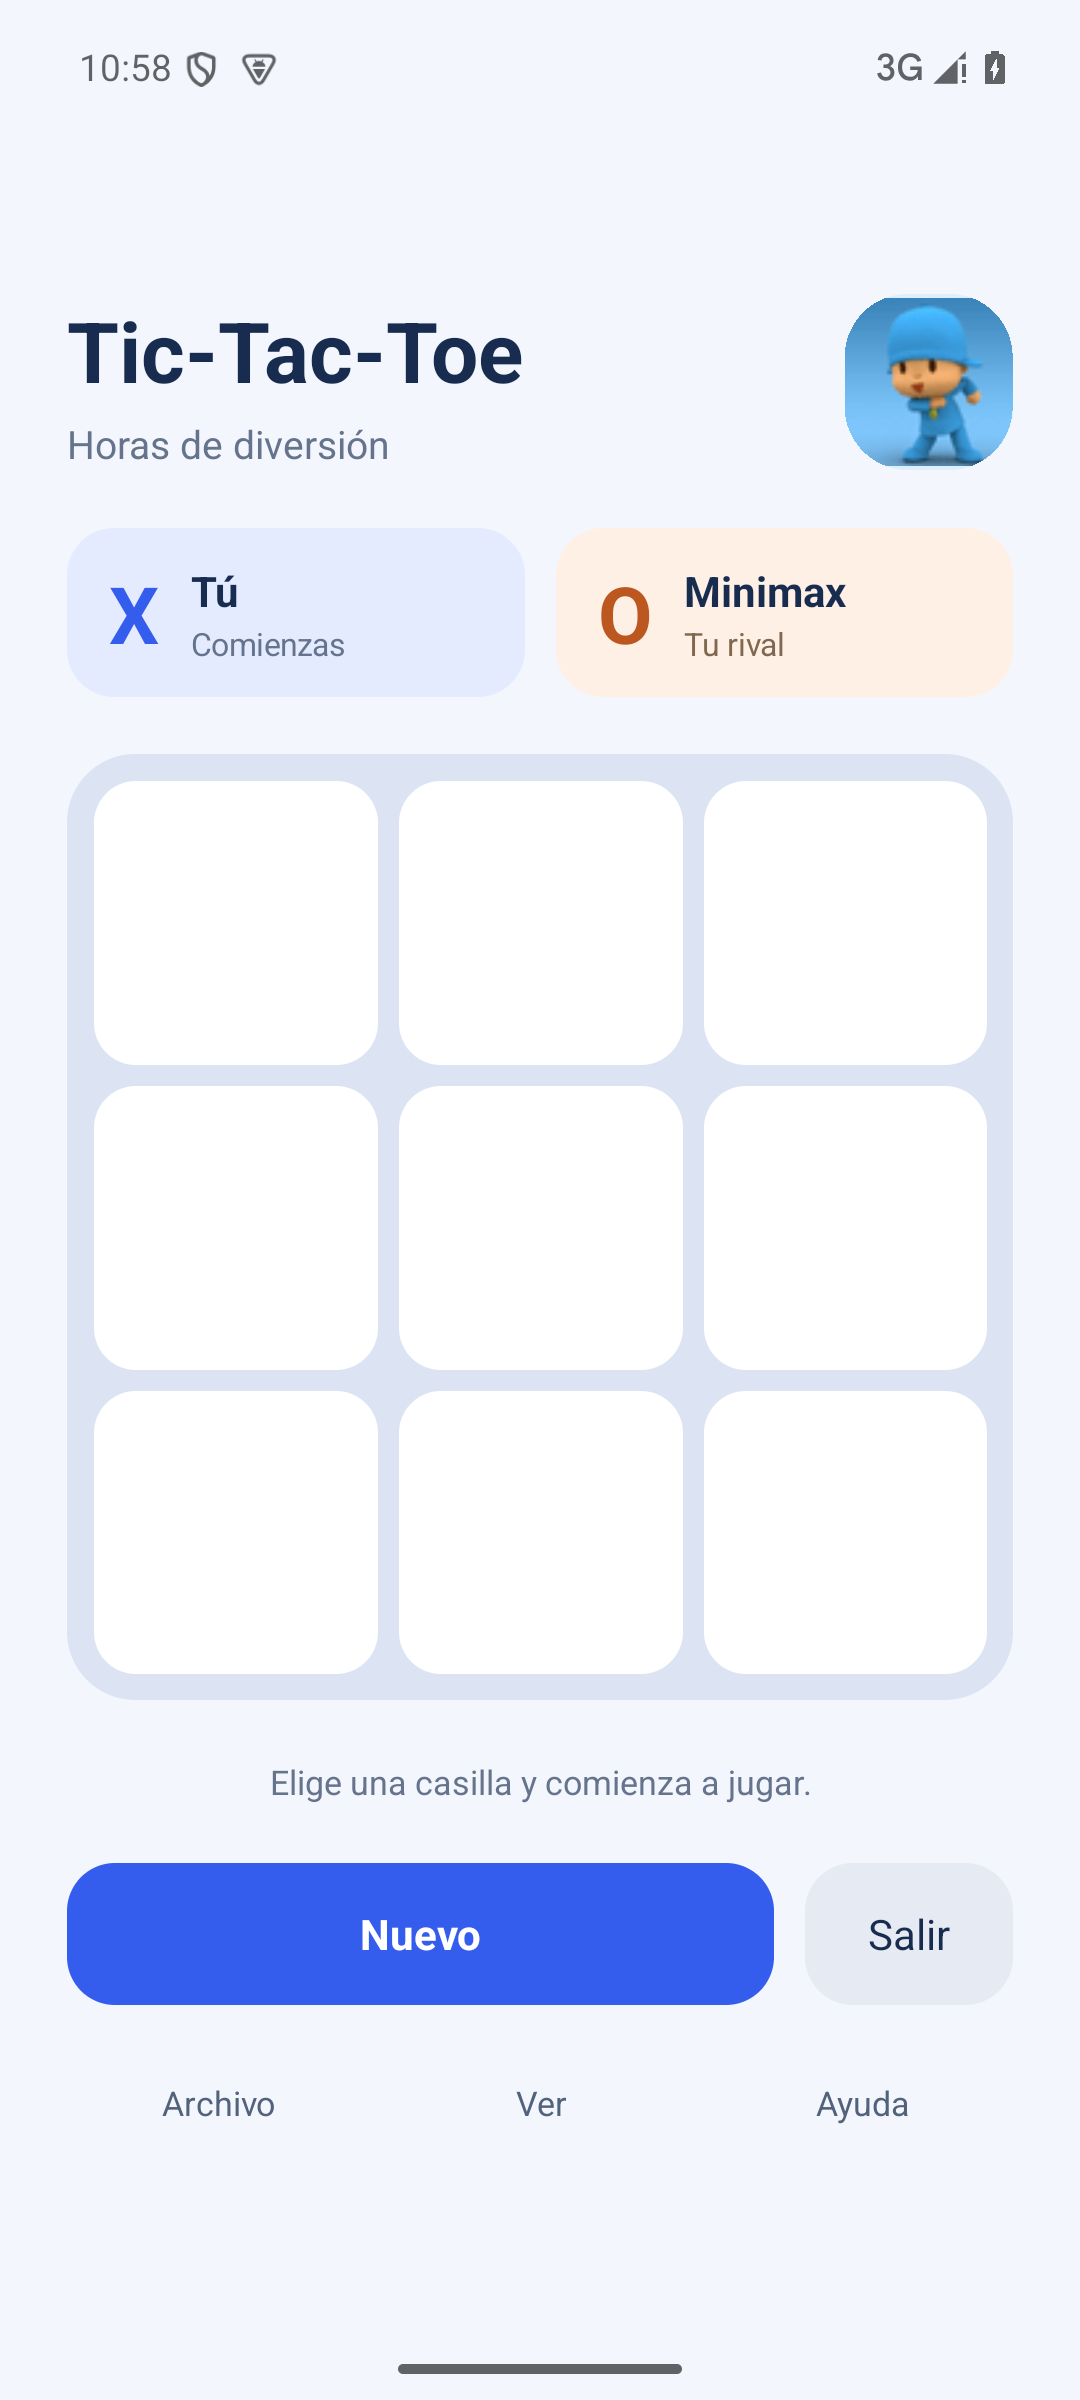
\includegraphics[height=0.65\textheight,keepaspectratio]{capturas_20261104_175826/01_inicio.png}
  \caption{Pantalla inicial: menús, personaje original, tablero vacío y botones Nuevo y Salir.}
  \label{fig:minmax-01}
\end{figure}

\begin{figure}[htbp]
  \centering
  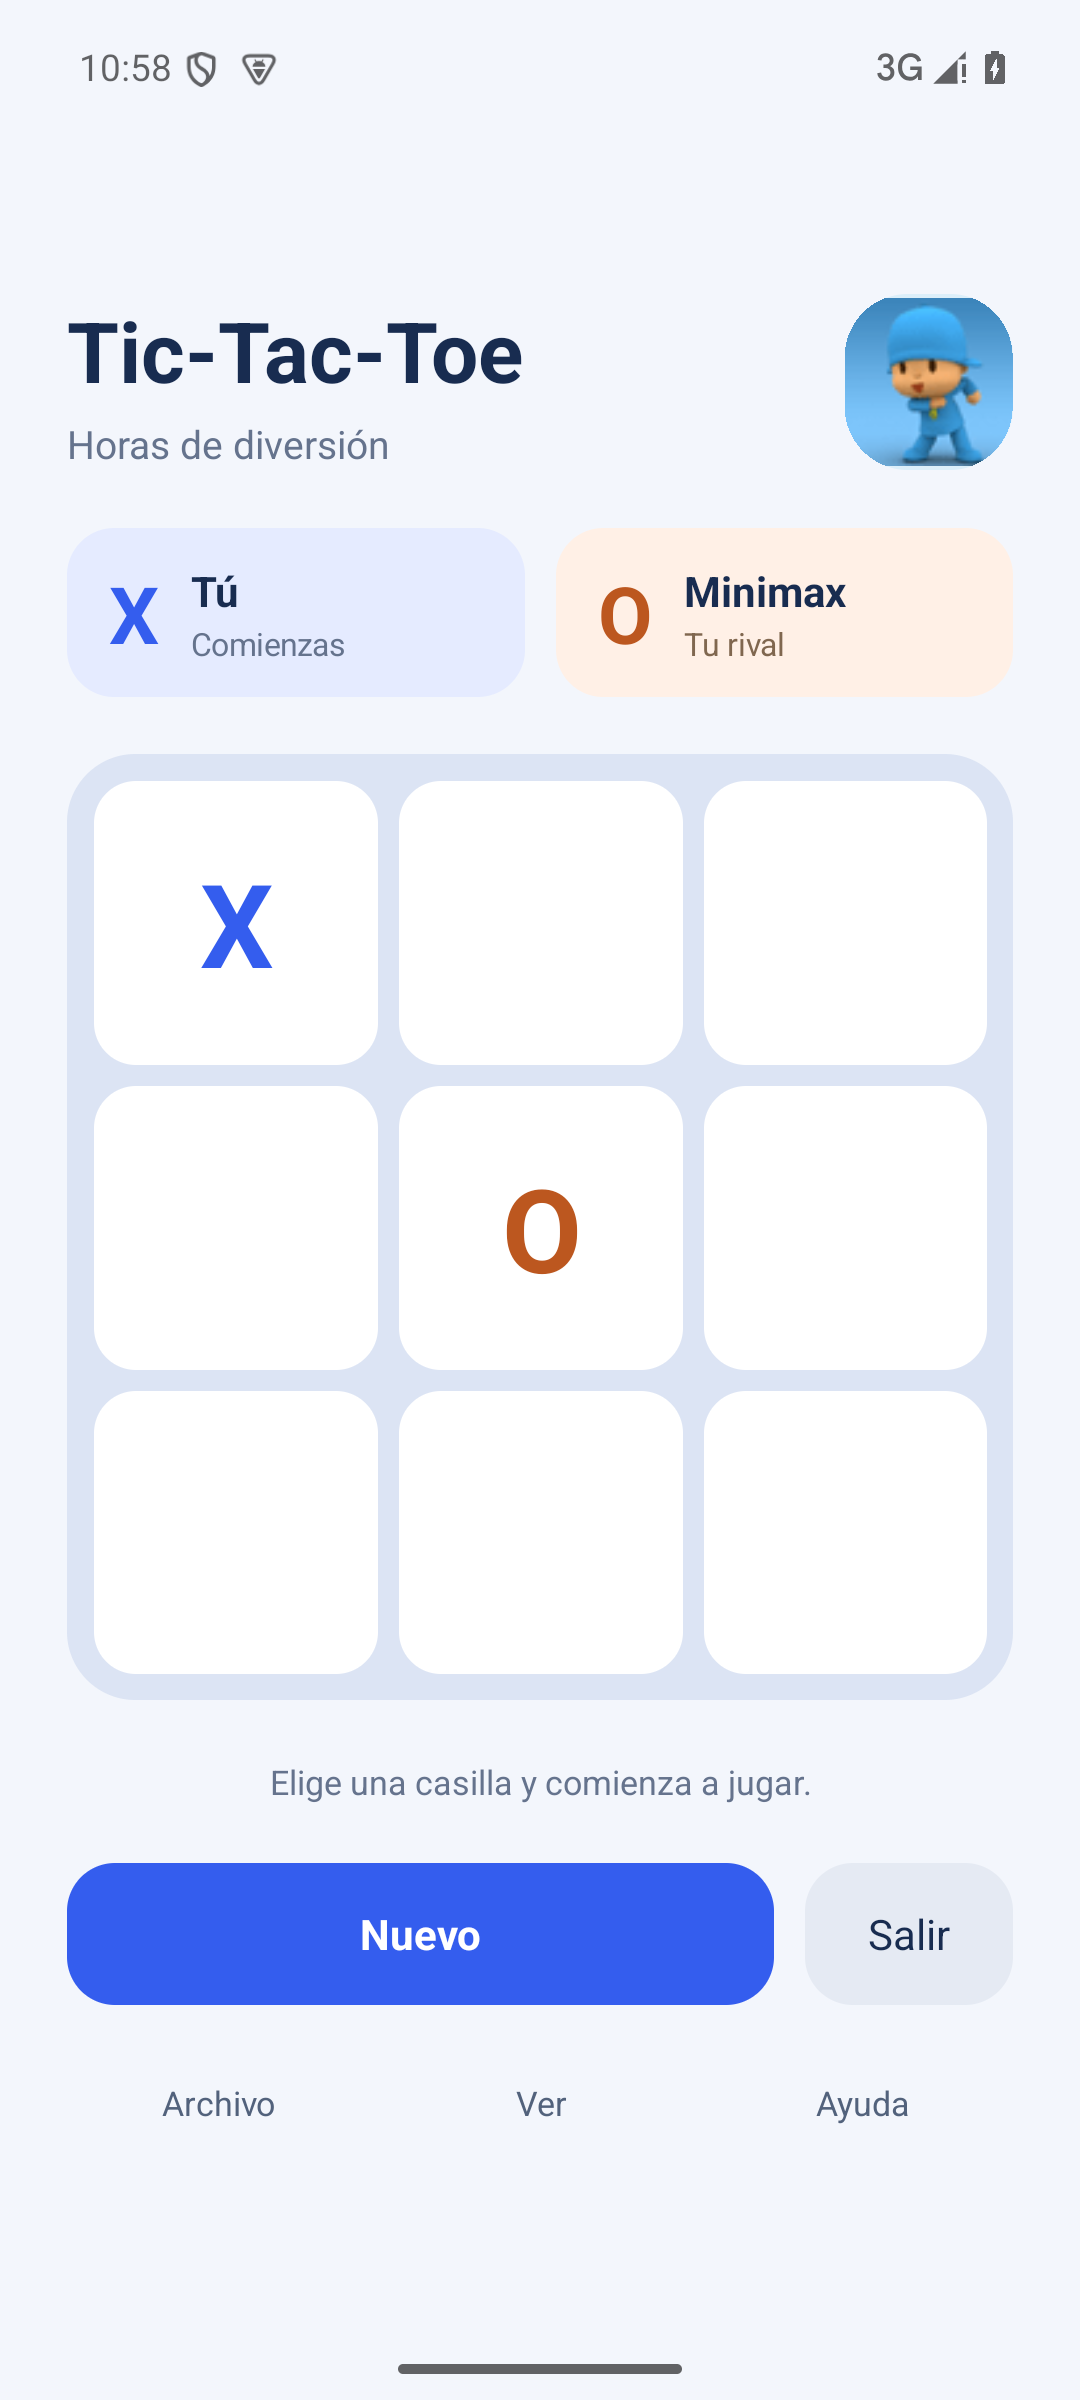
\includegraphics[height=0.65\textheight,keepaspectratio]{capturas_20261104_175826/02_turno_humano_ia.png}
  \caption{Jugada humana X y respuesta automática O de Minimax.}
  \label{fig:minmax-02}
\end{figure}

\begin{figure}[htbp]
  \centering
  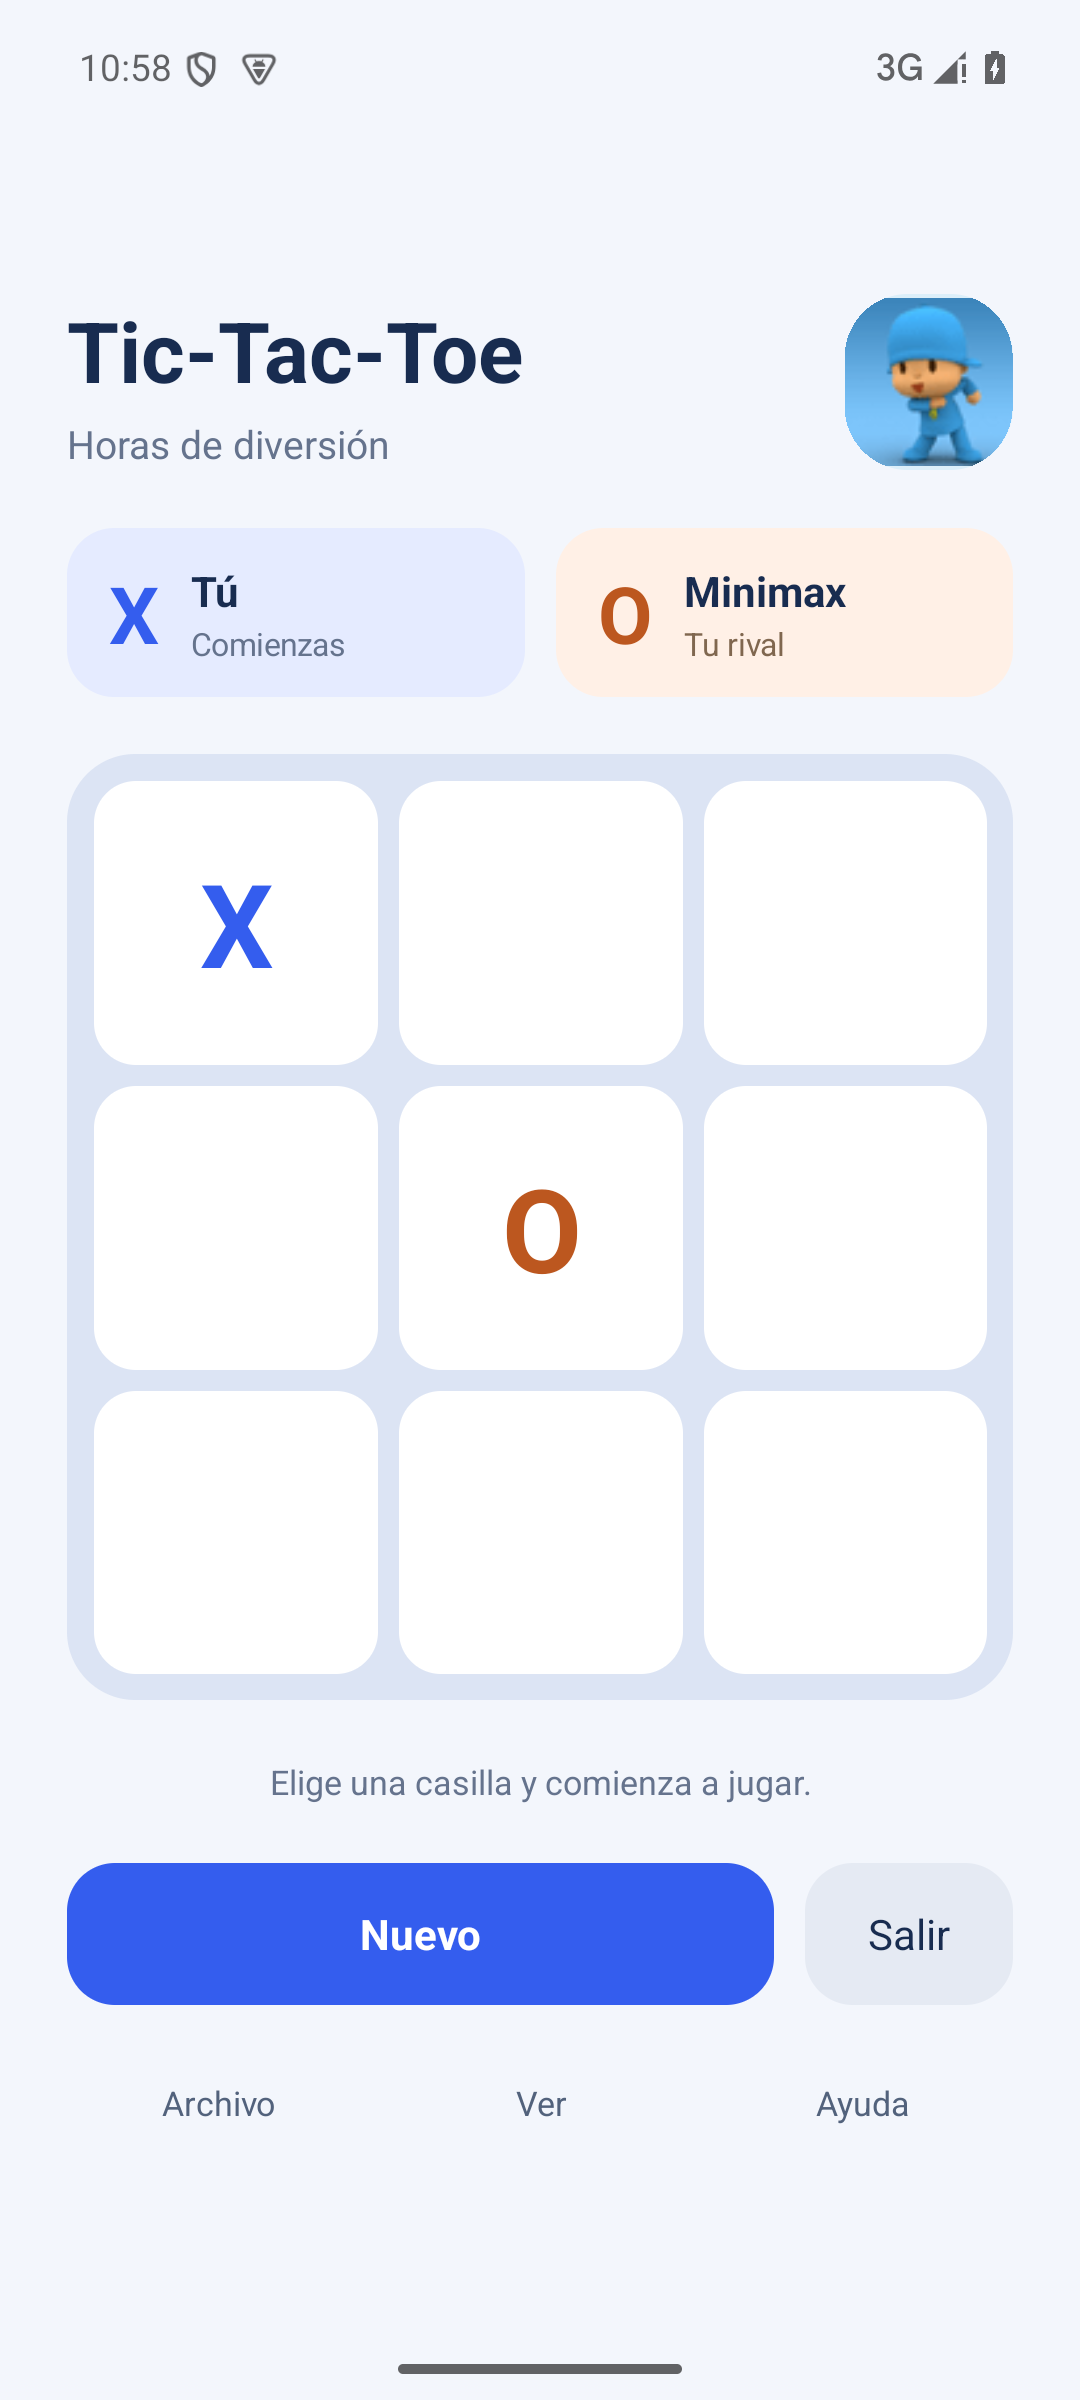
\includegraphics[height=0.65\textheight,keepaspectratio]{capturas_20261104_175826/03_casilla_ocupada.png}
  \caption{El tablero se conserva tras pulsar una casilla ocupada.}
  \label{fig:minmax-03}
\end{figure}

\begin{figure}[htbp]
  \centering
  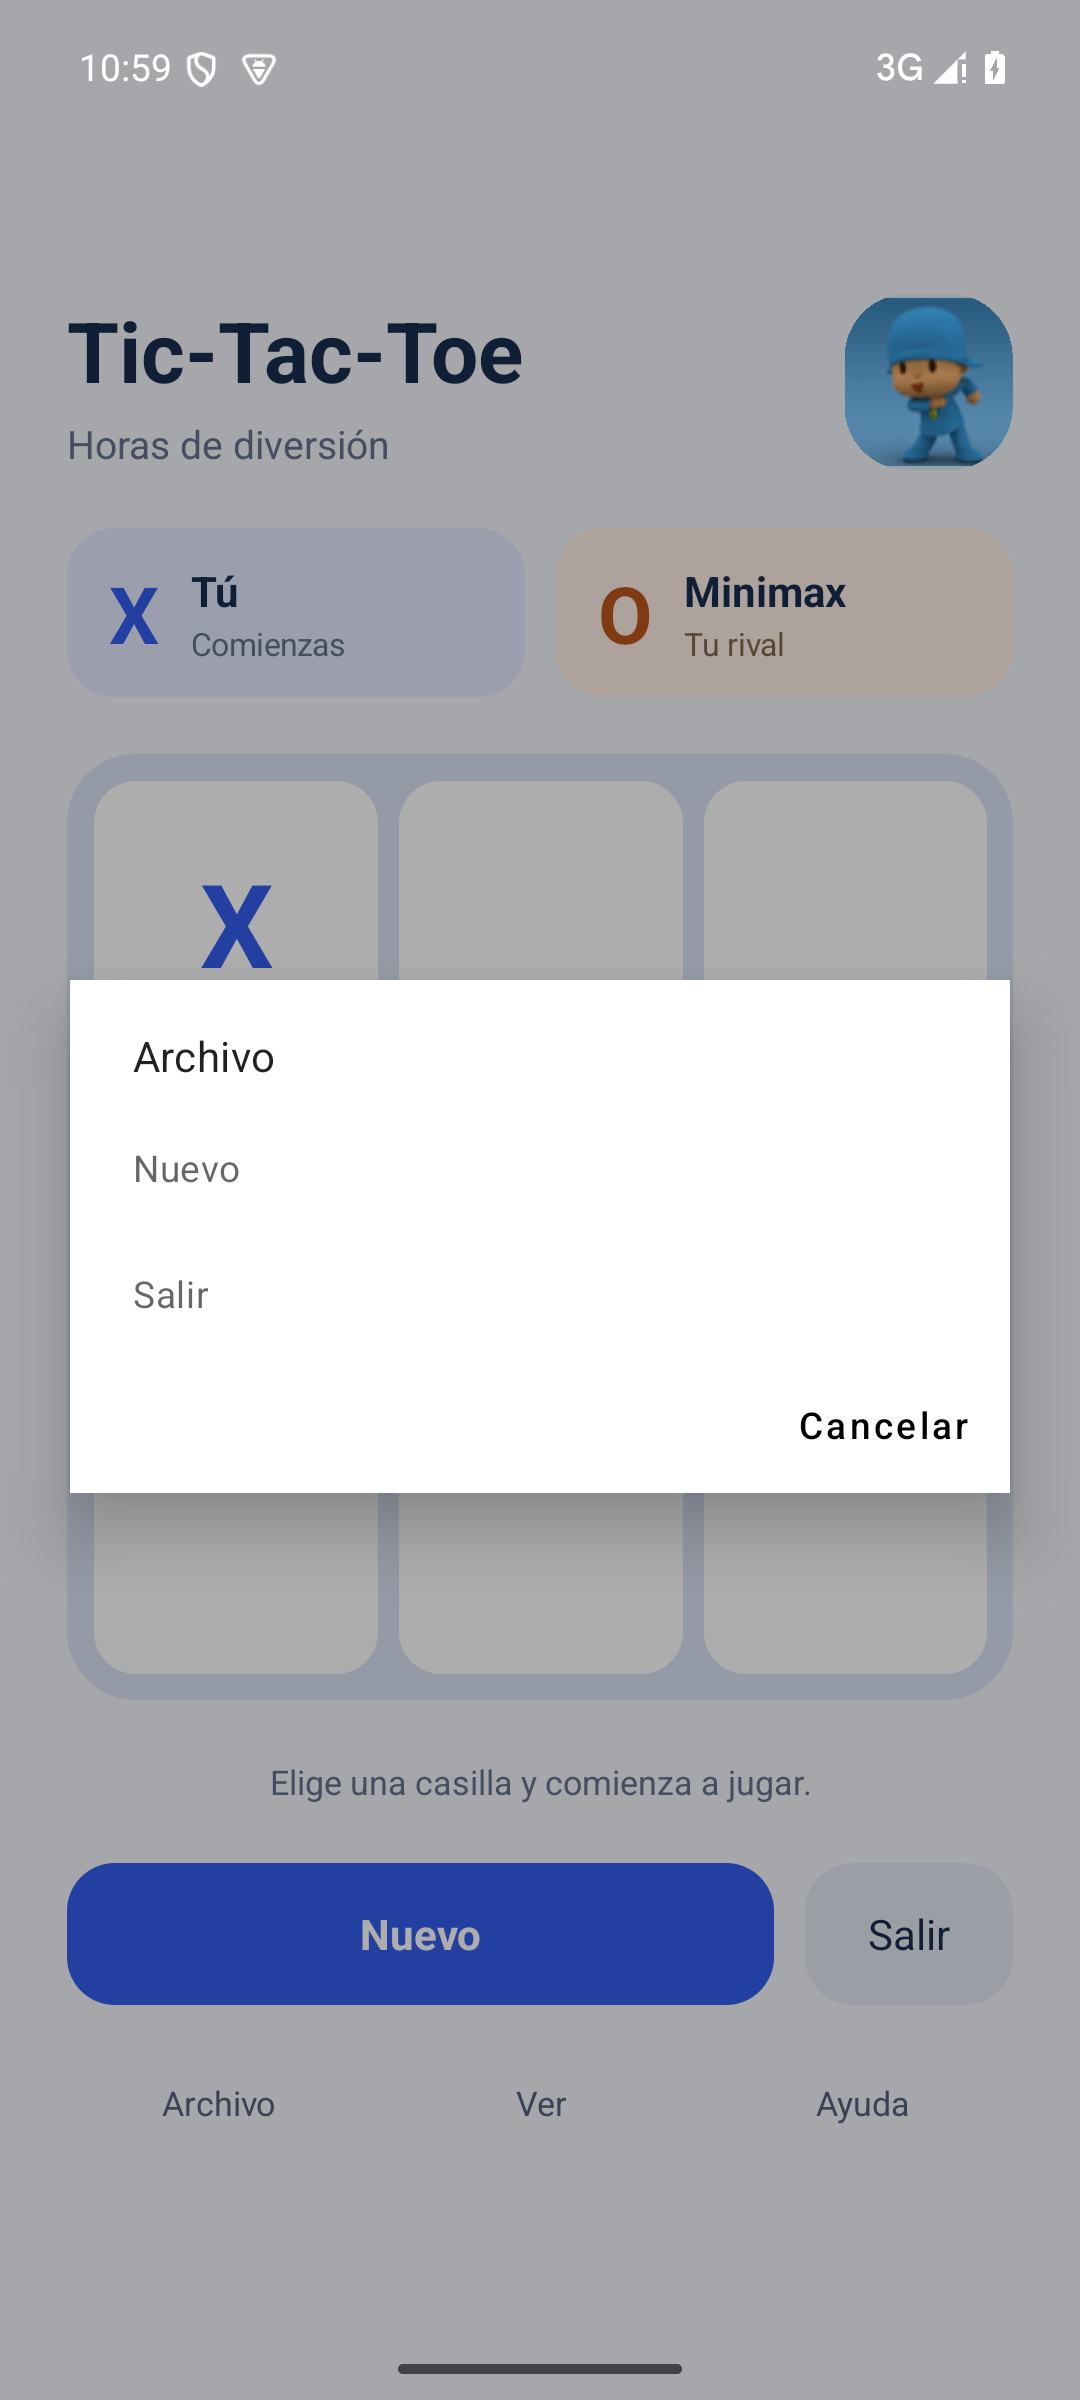
\includegraphics[height=0.65\textheight,keepaspectratio]{capturas_20261104_175826/04_menu_archivo.png}
  \caption{Menú Archivo con las opciones del proyecto WinForms original.}
  \label{fig:minmax-04}
\end{figure}

\begin{figure}[htbp]
  \centering
  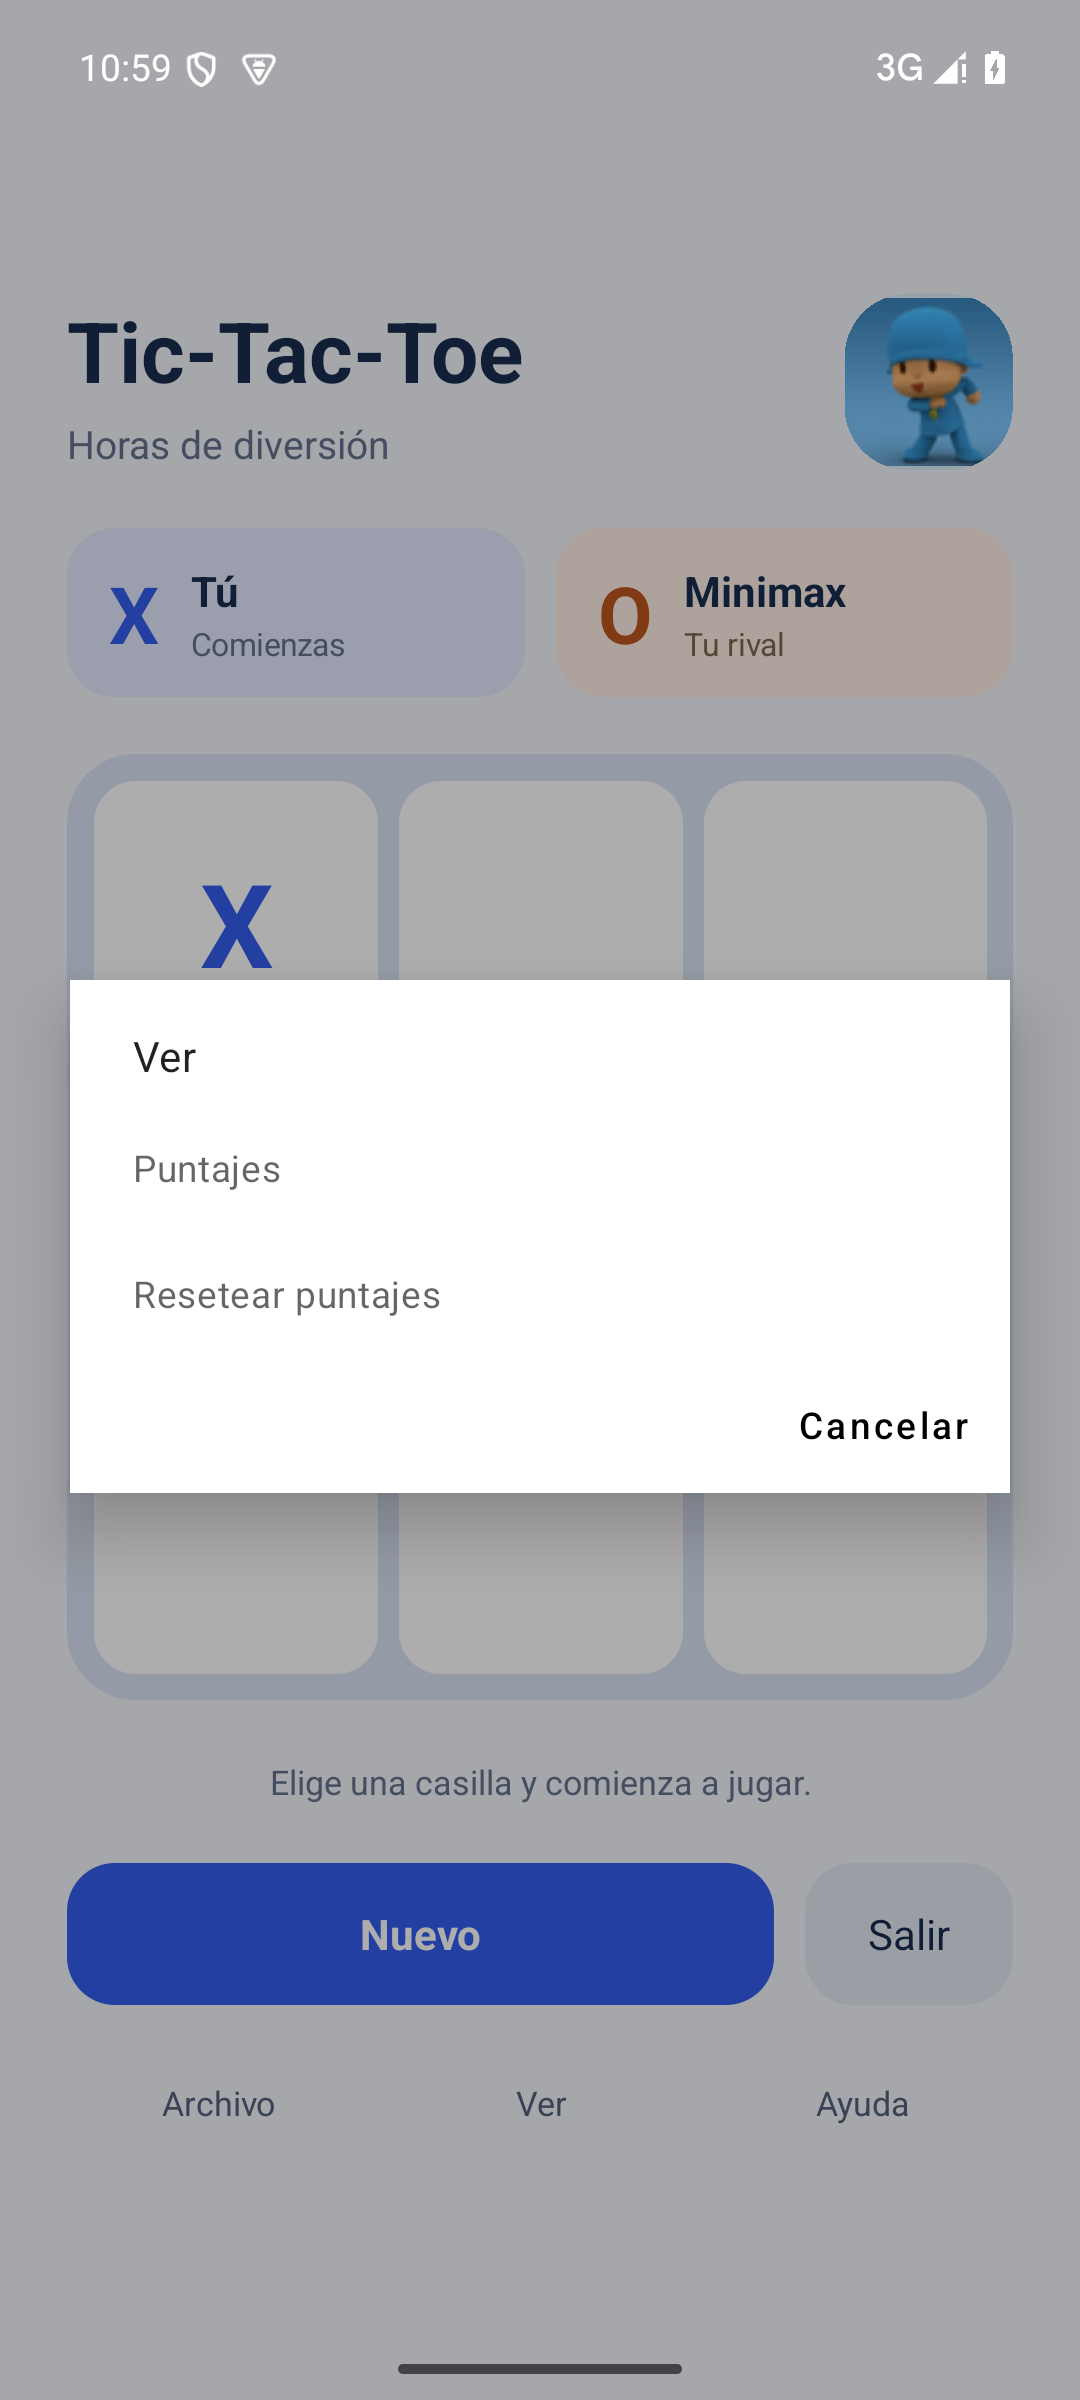
\includegraphics[height=0.65\textheight,keepaspectratio]{capturas_20261104_175826/05_menu_ver.png}
  \caption{Menú Ver con las opciones del proyecto WinForms original.}
  \label{fig:minmax-05}
\end{figure}

\begin{figure}[htbp]
  \centering
  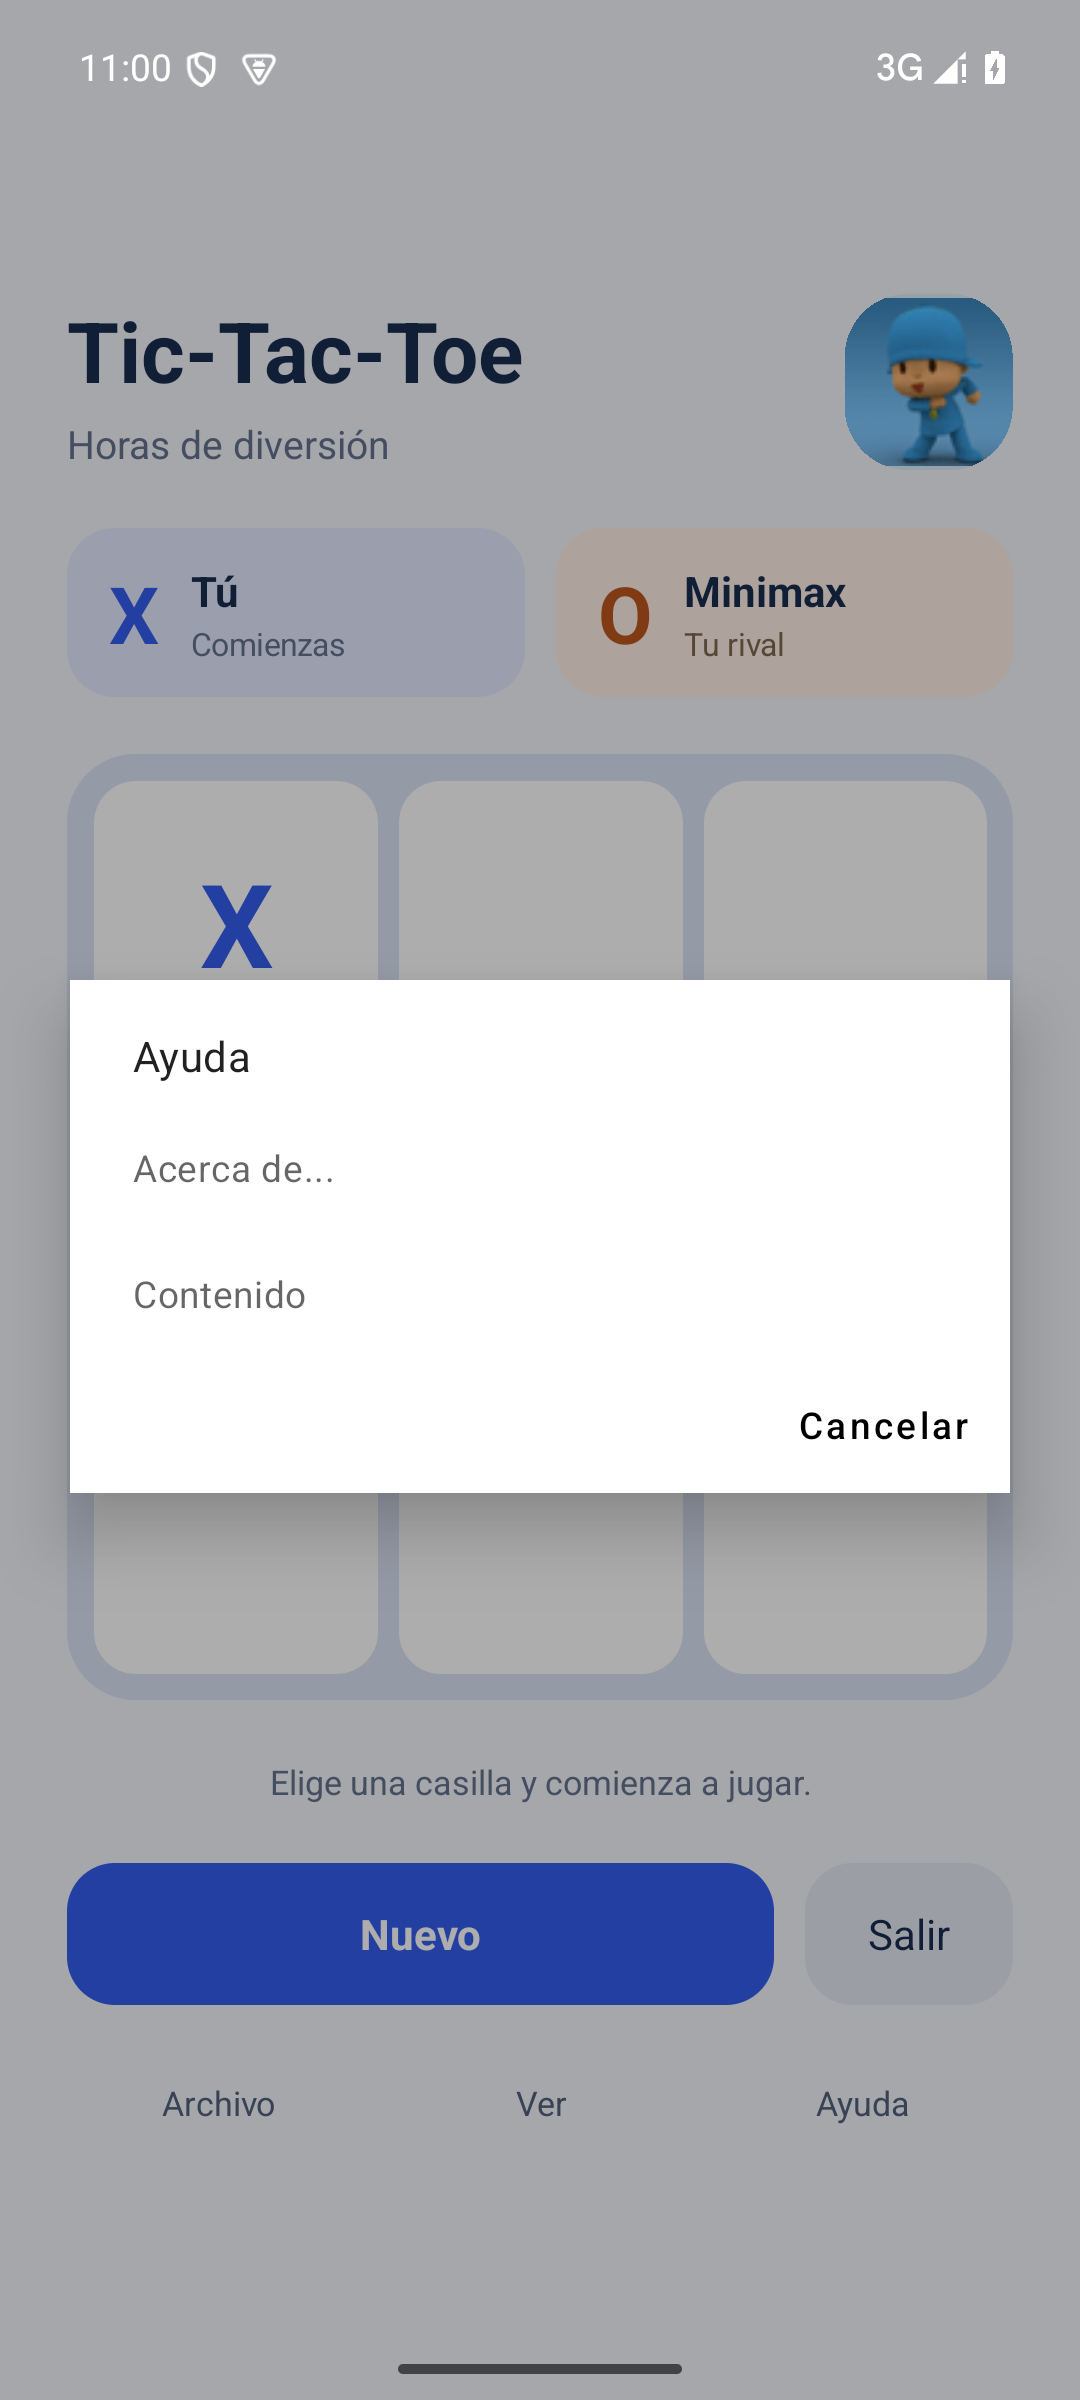
\includegraphics[height=0.65\textheight,keepaspectratio]{capturas_20261104_175826/06_menu_ayuda.png}
  \caption{Menú Ayuda con las opciones del proyecto WinForms original.}
  \label{fig:minmax-06}
\end{figure}

\begin{figure}[htbp]
  \centering
  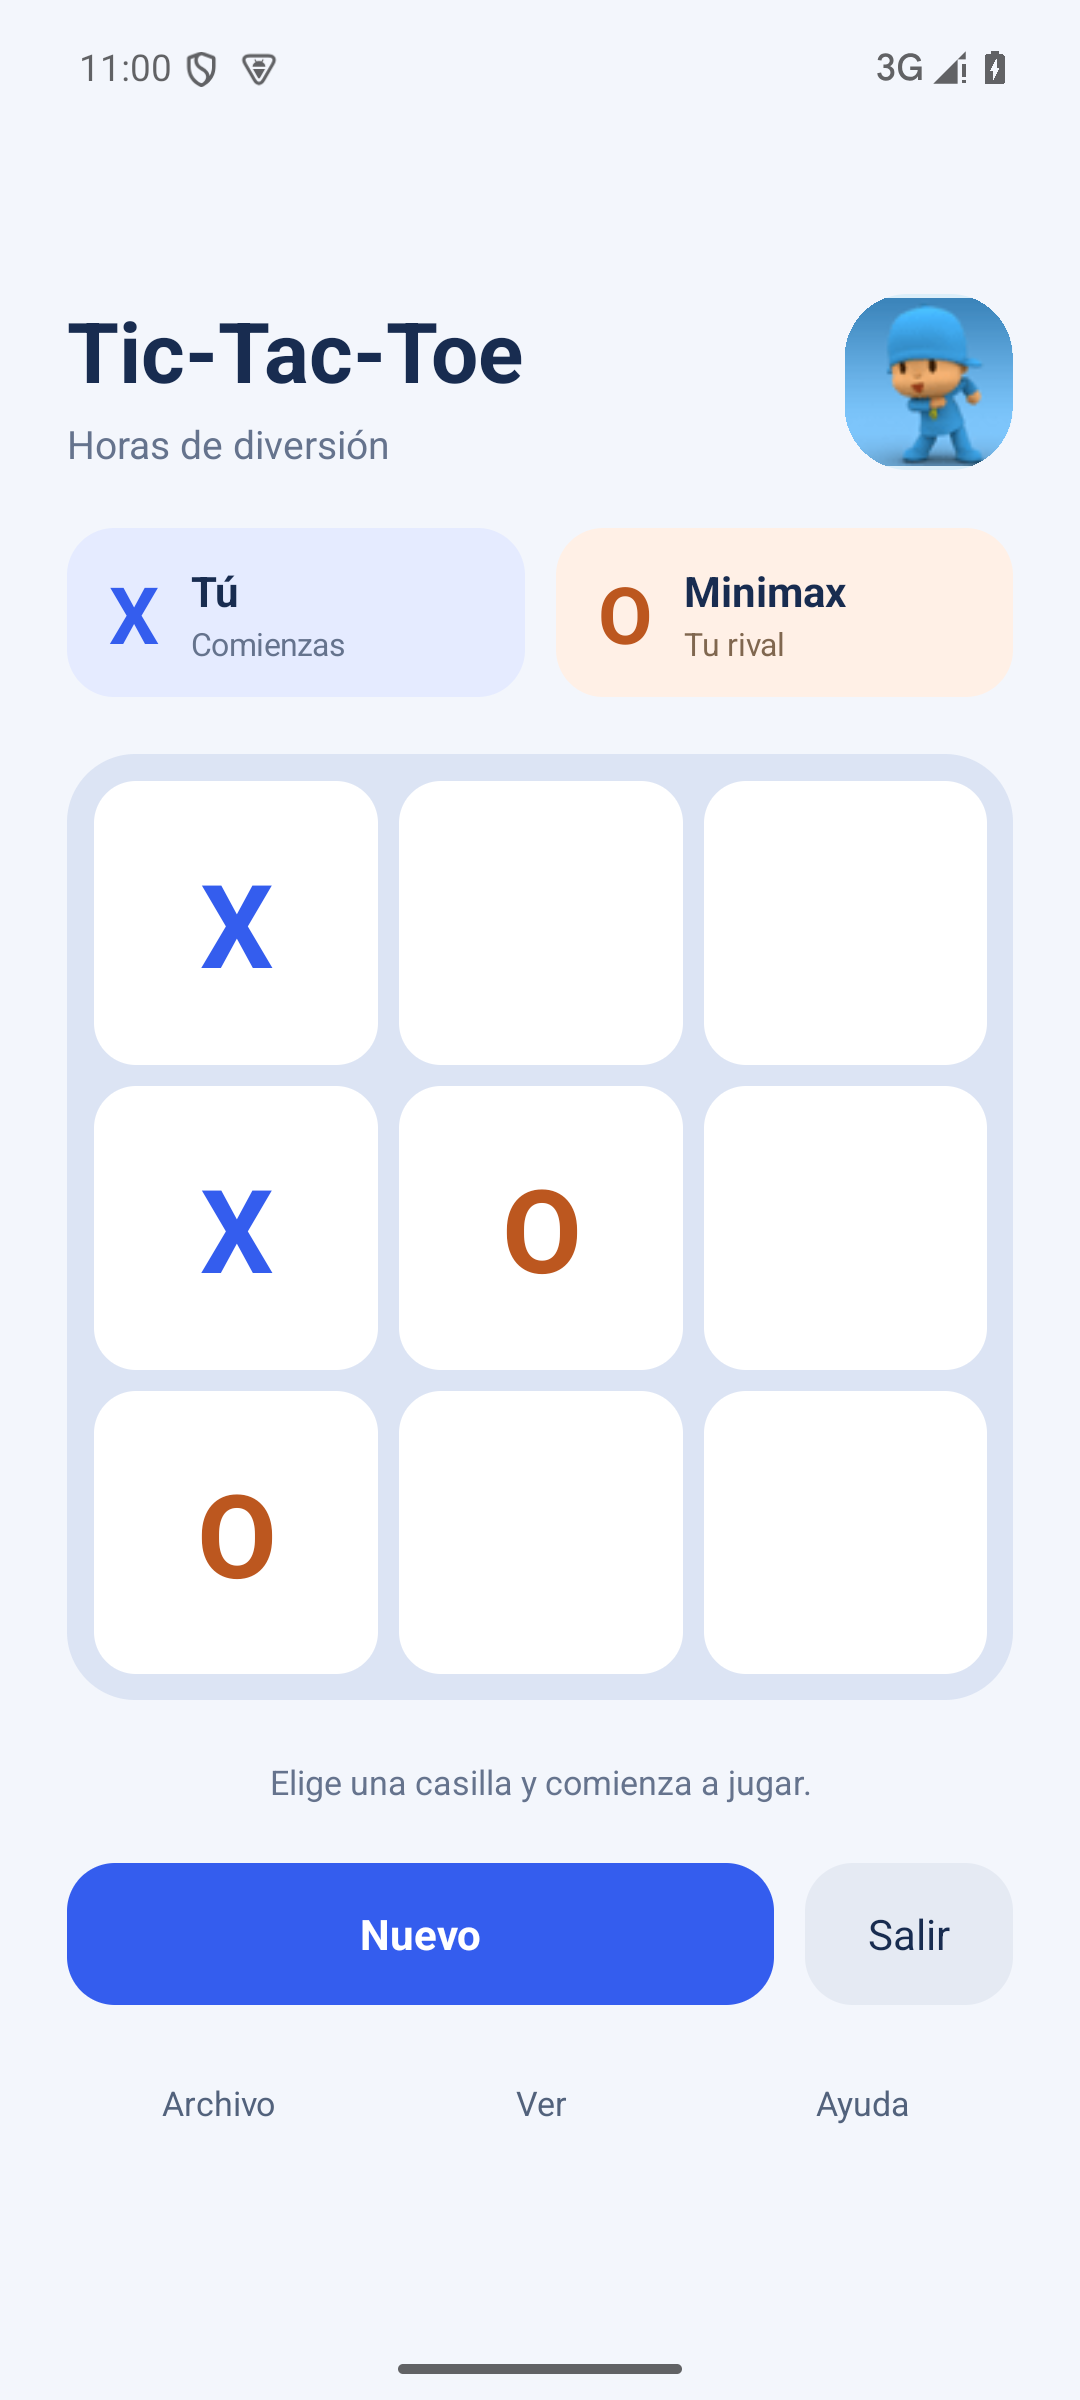
\includegraphics[height=0.65\textheight,keepaspectratio]{capturas_20261104_175826/07_ia_bloquea.png}
  \caption{Minimax bloquea la amenaza de victoria de X en la primera columna.}
  \label{fig:minmax-07}
\end{figure}

\begin{figure}[htbp]
  \centering
  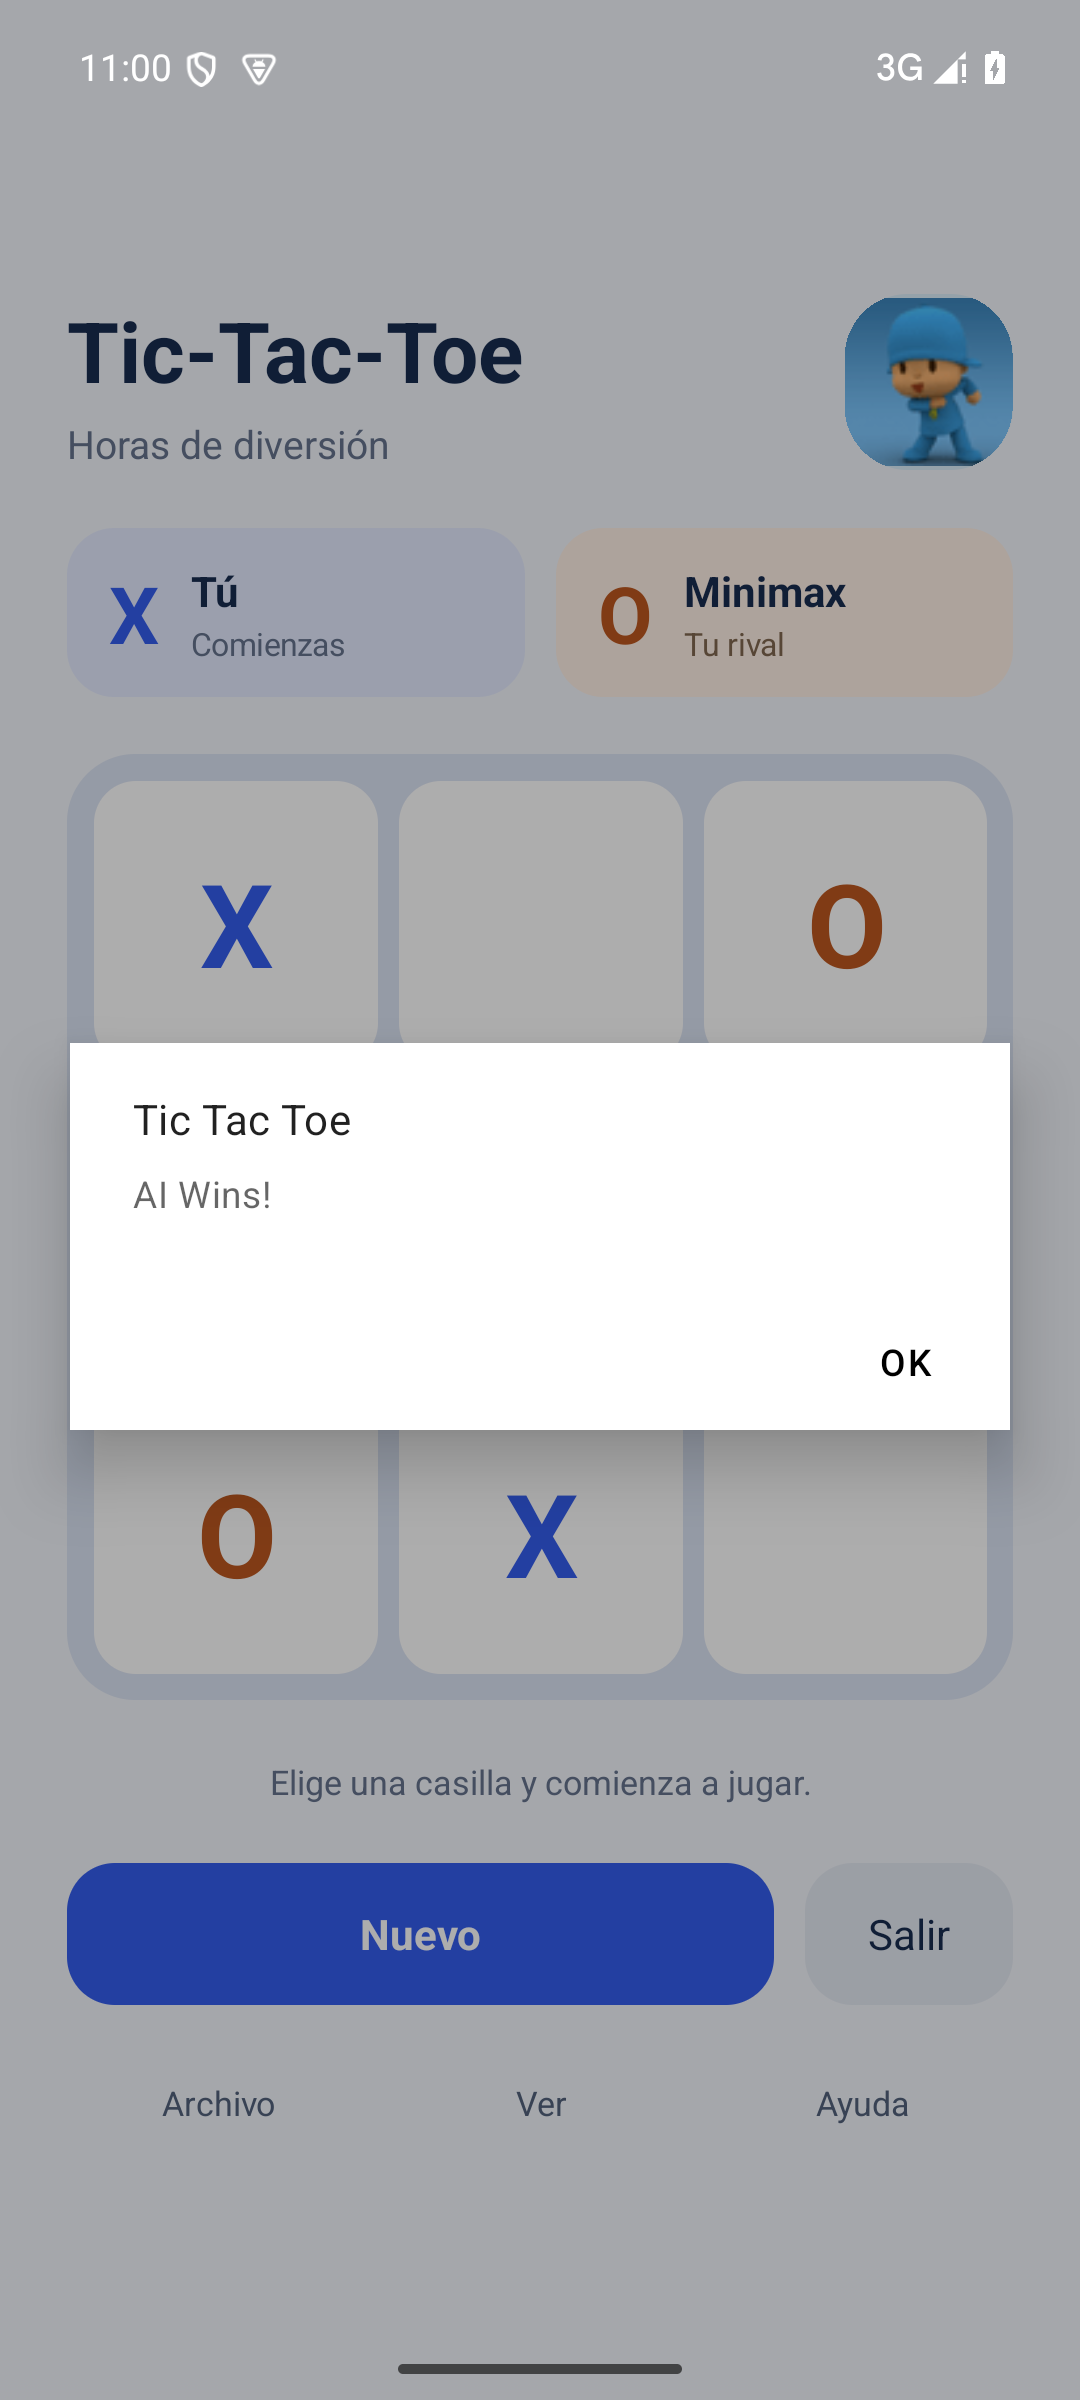
\includegraphics[height=0.65\textheight,keepaspectratio]{capturas_20261104_175826/08_victoria_ia.png}
  \caption{Aviso original de victoria de la IA.}
  \label{fig:minmax-08}
\end{figure}

\begin{figure}[htbp]
  \centering
  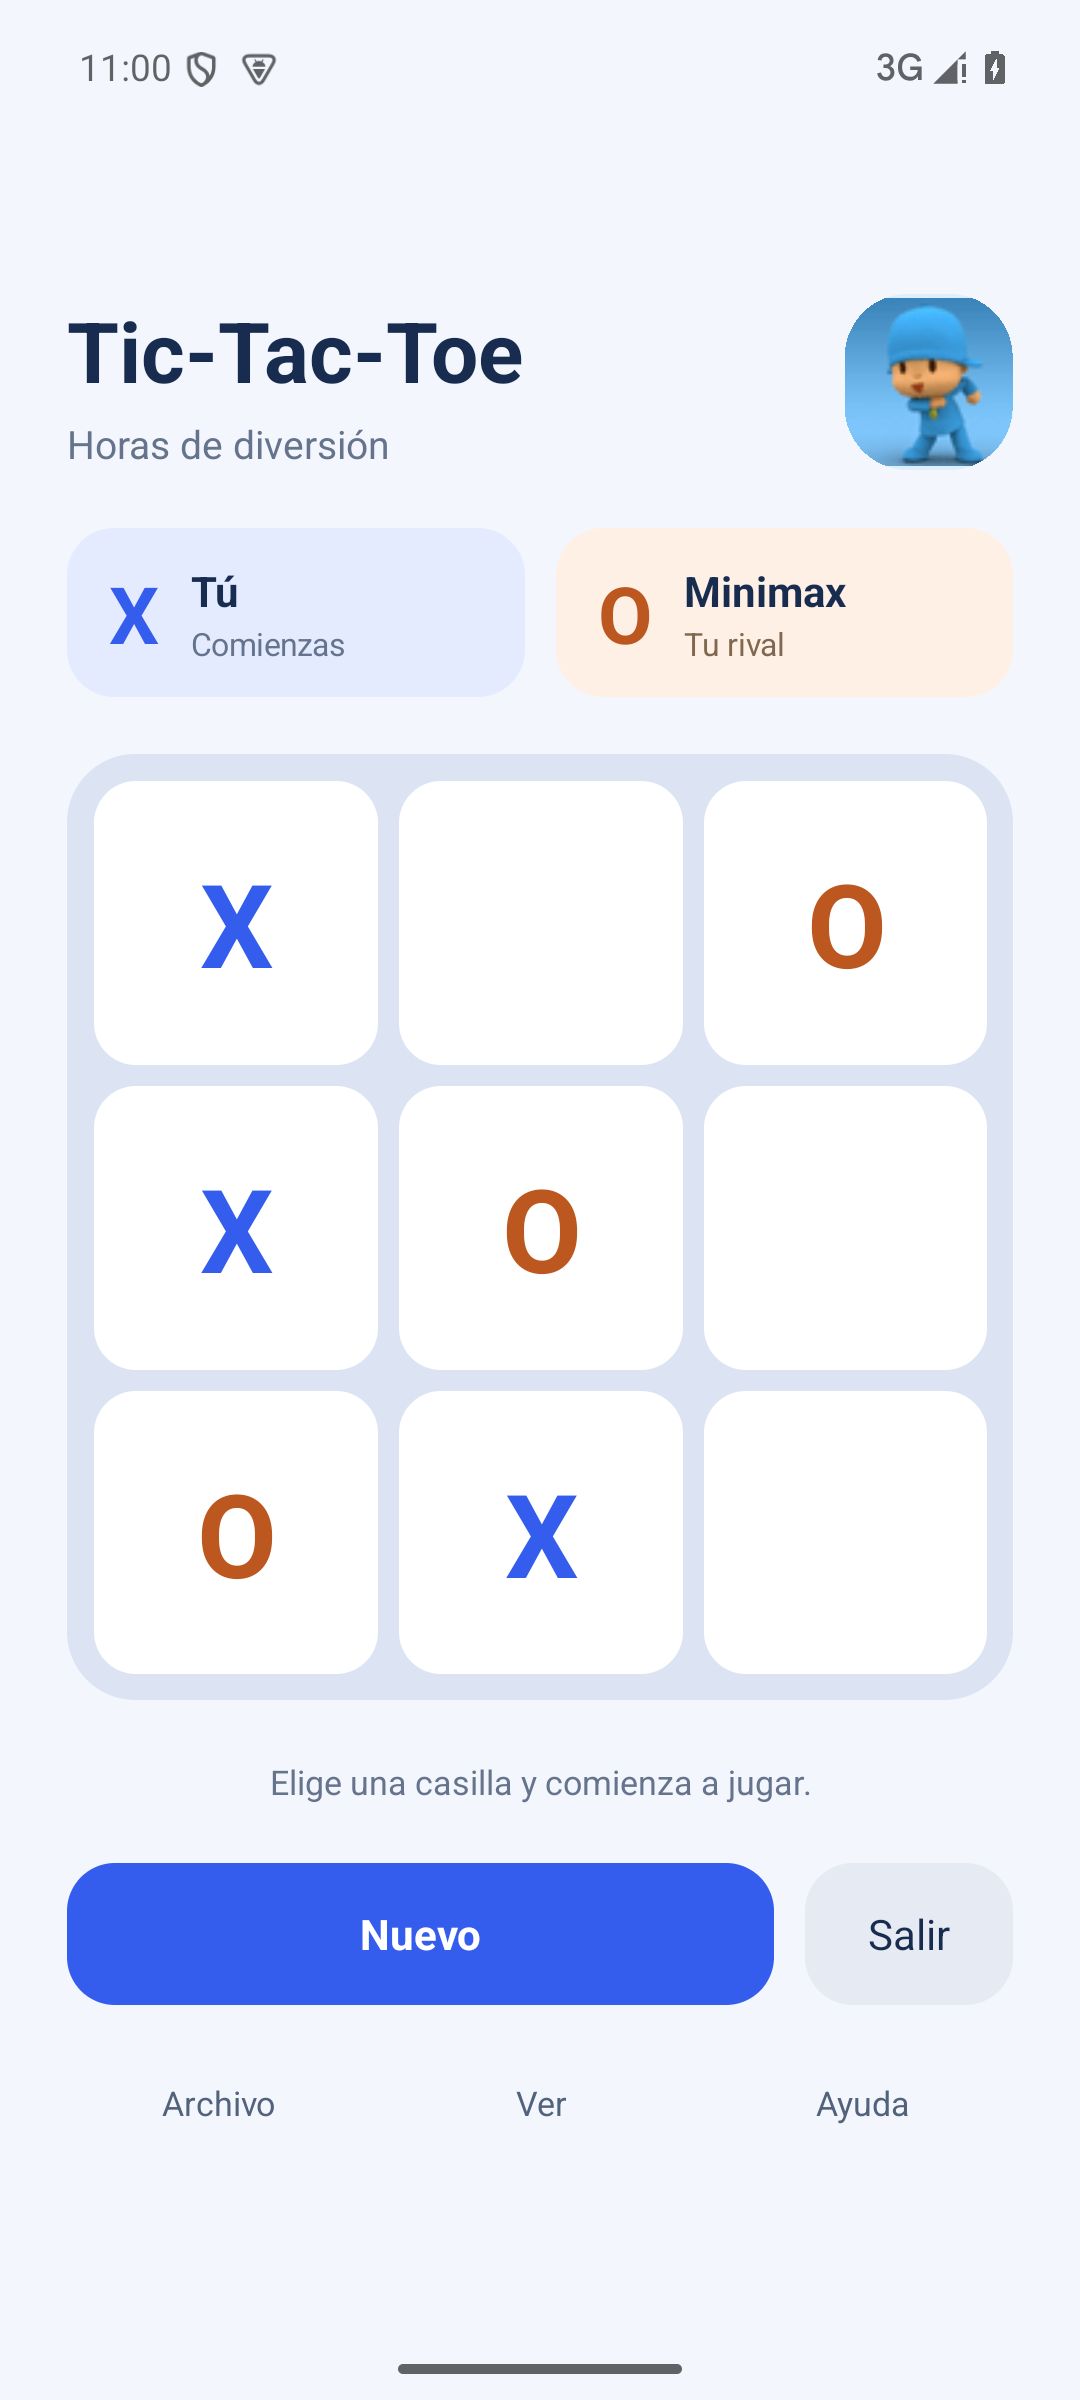
\includegraphics[height=0.65\textheight,keepaspectratio]{capturas_20261104_175826/09_partida_finalizada.png}
  \caption{Diagonal ganadora de O y tablero bloqueado al finalizar.}
  \label{fig:minmax-09}
\end{figure}

\begin{figure}[htbp]
  \centering
  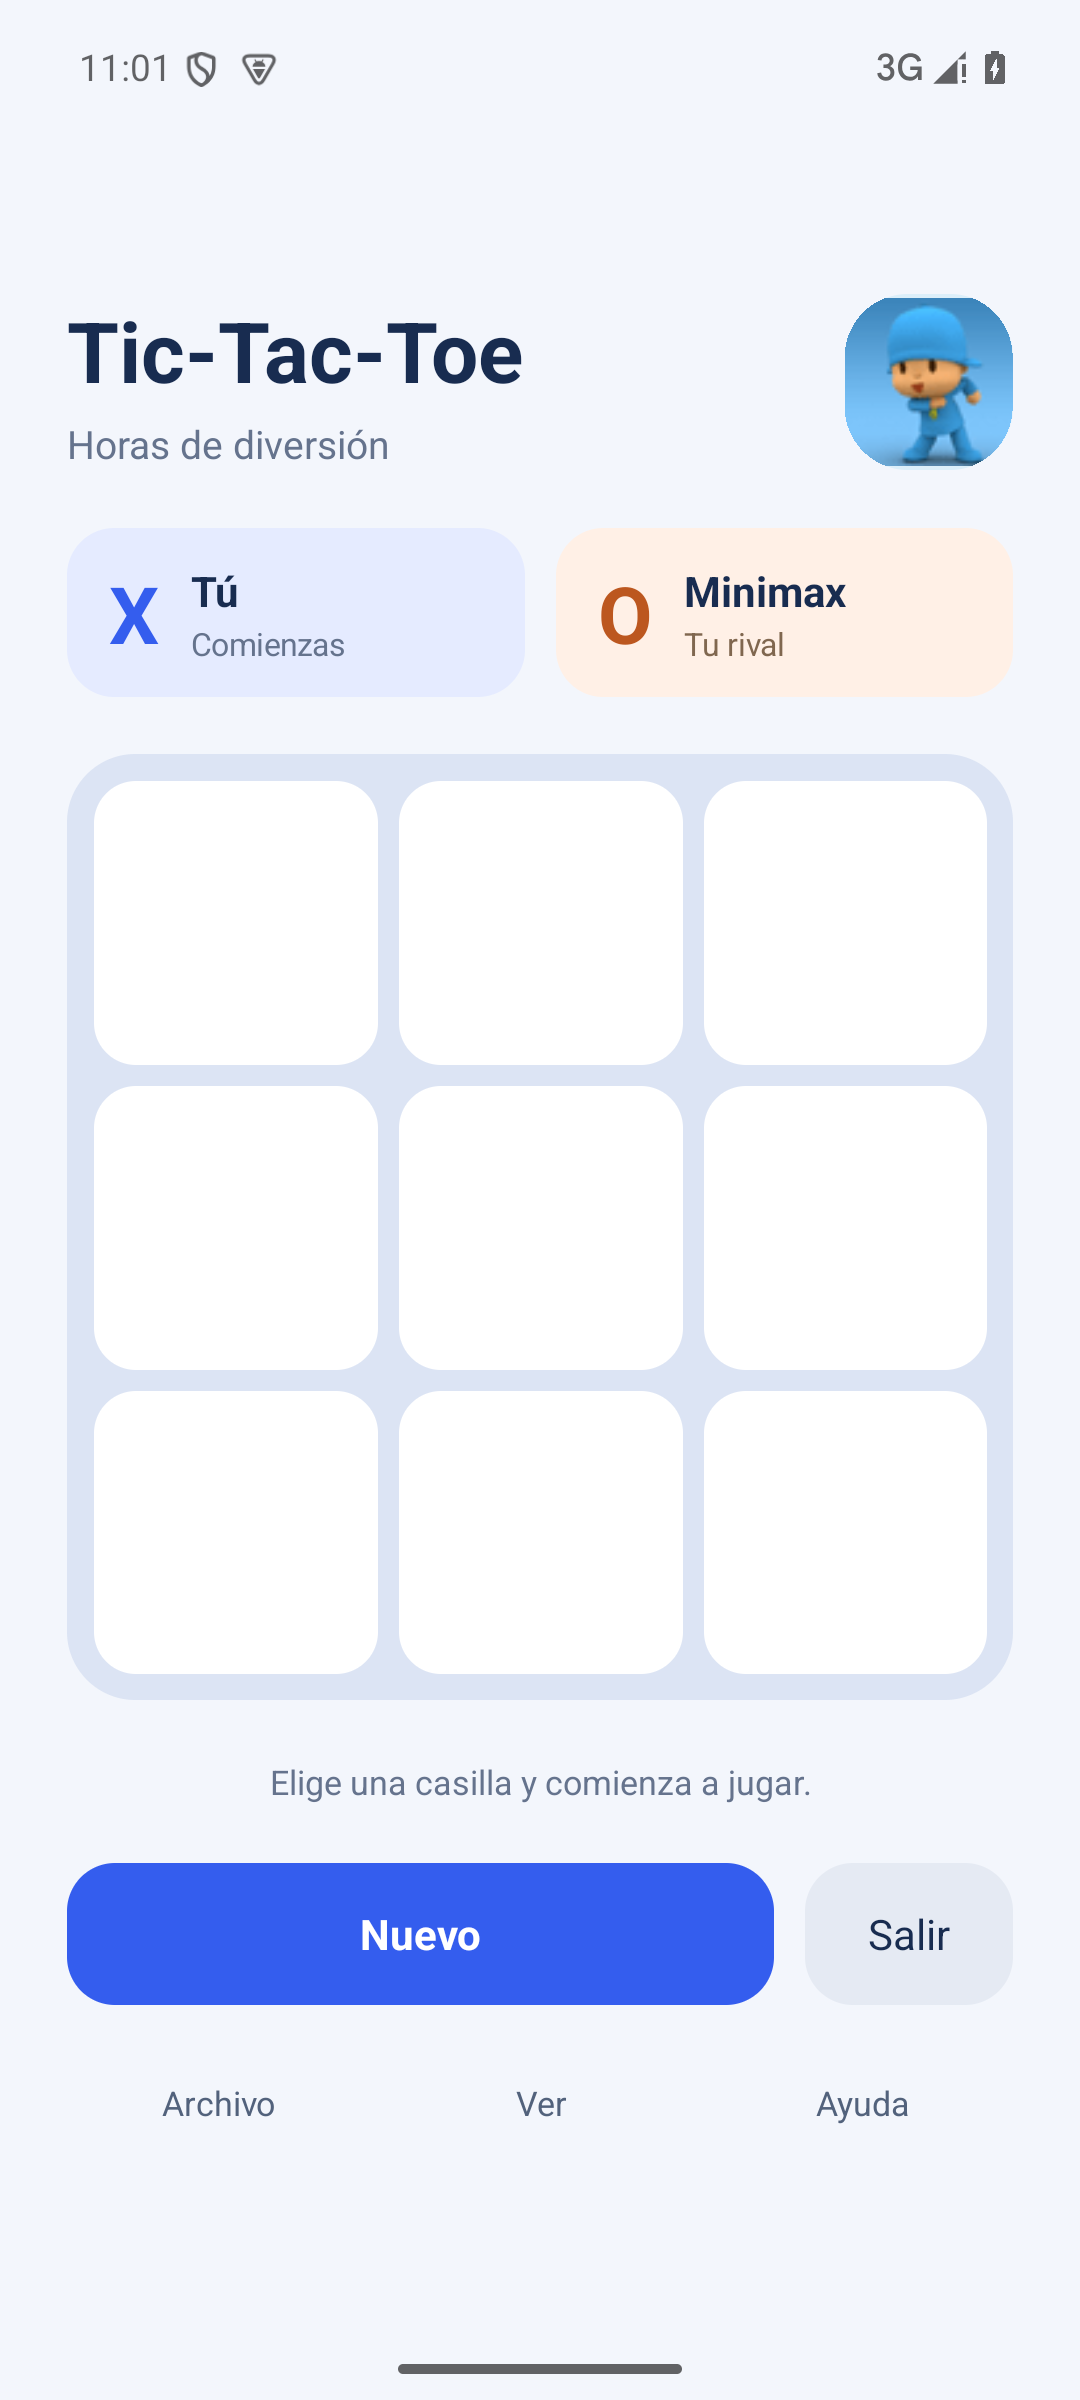
\includegraphics[height=0.65\textheight,keepaspectratio]{capturas_20261104_175826/10_reinicio.png}
  \caption{Nuevo borra la partida terminada y vuelve a habilitar las nueve casillas.}
  \label{fig:minmax-10}
\end{figure}

\begin{figure}[htbp]
  \centering
  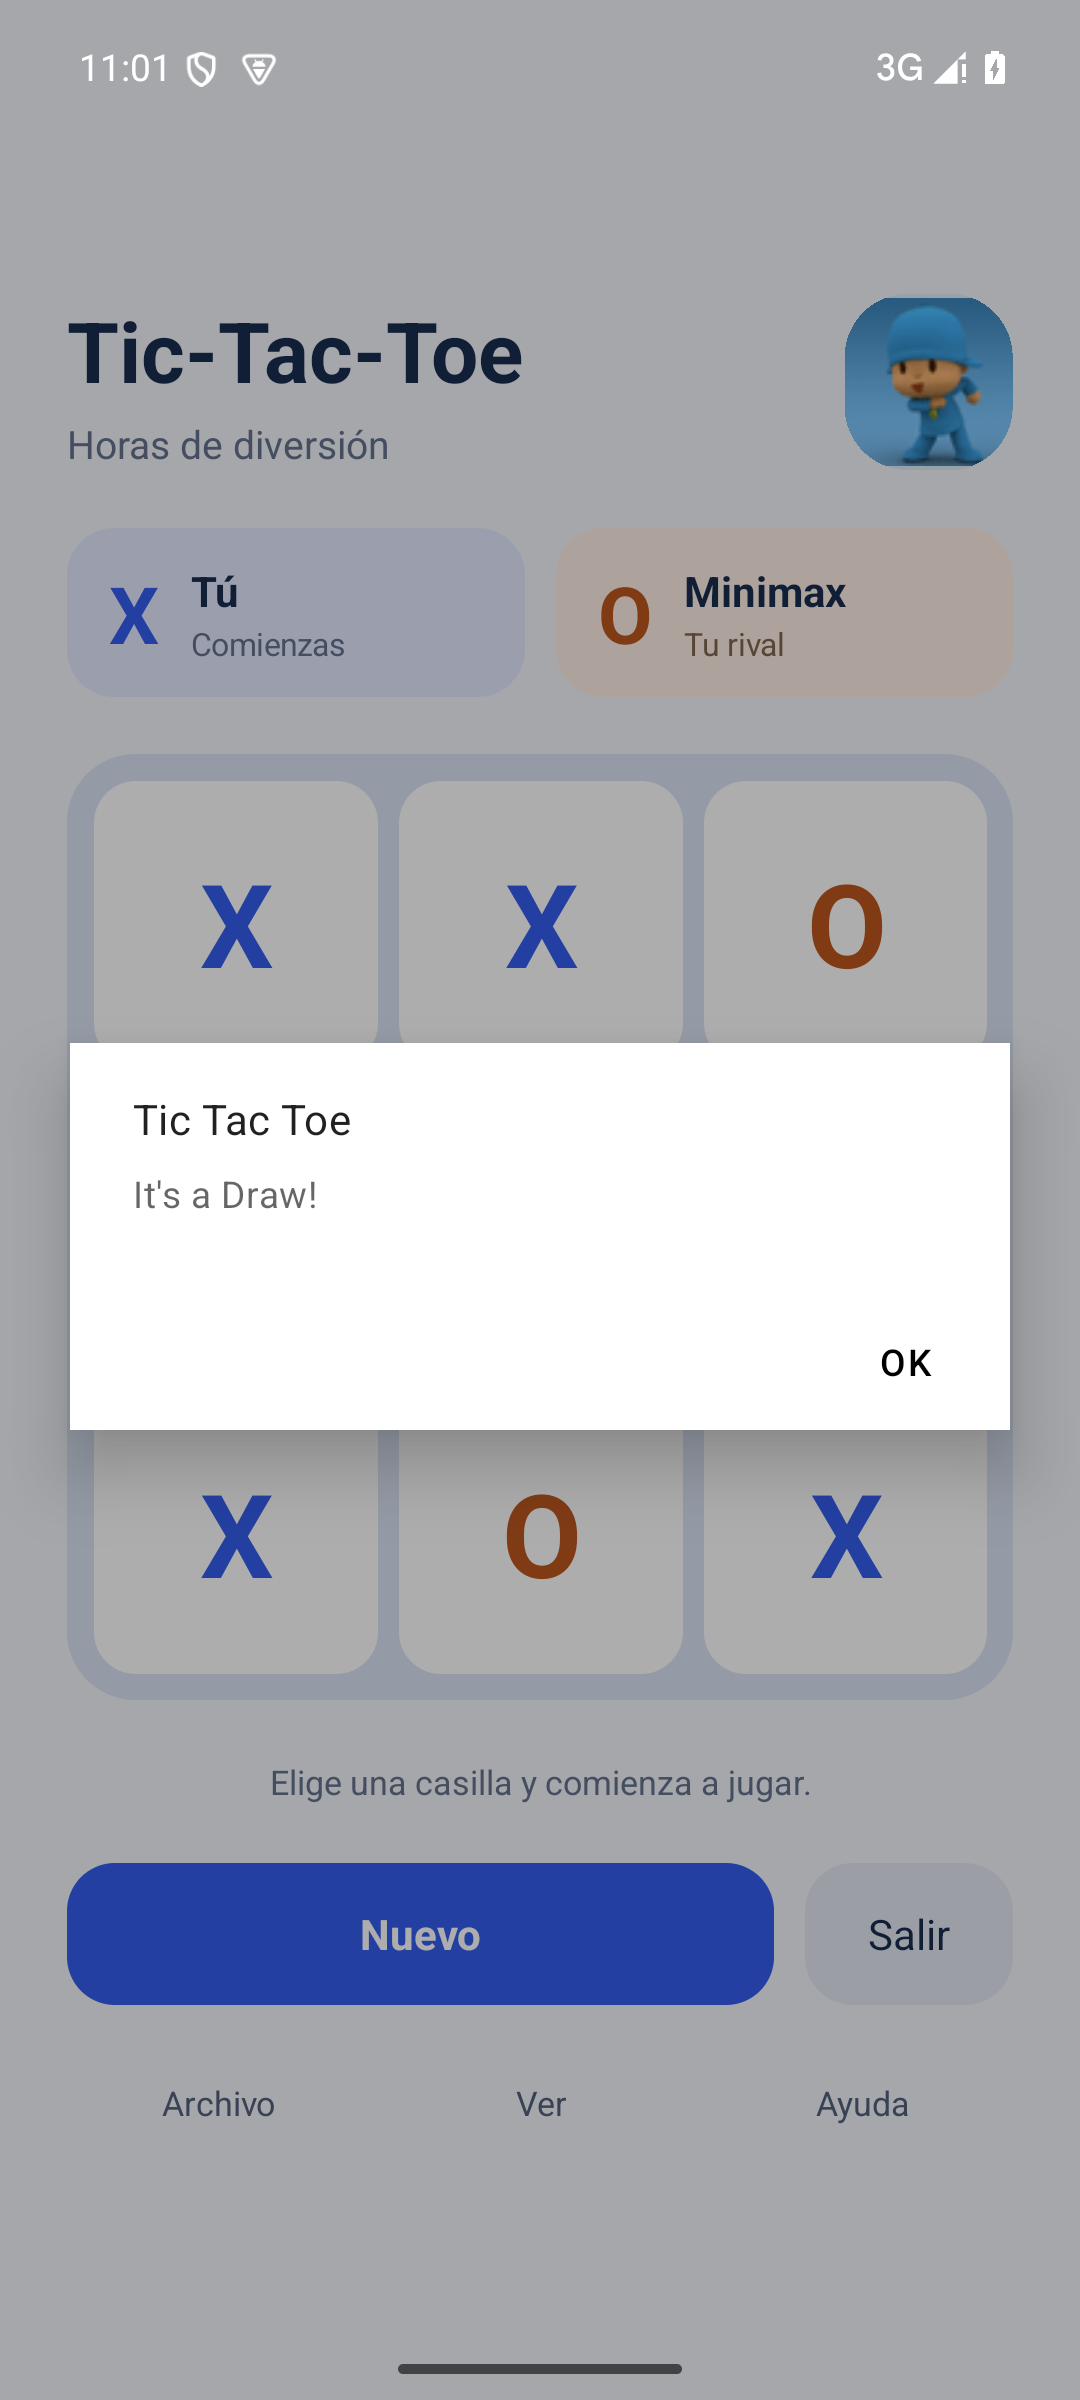
\includegraphics[height=0.65\textheight,keepaspectratio]{capturas_20261104_175826/11_empate_aviso.png}
  \caption{Aviso original de empate después de llenar el tablero sin ganador.}
  \label{fig:minmax-11}
\end{figure}

\begin{figure}[htbp]
  \centering
  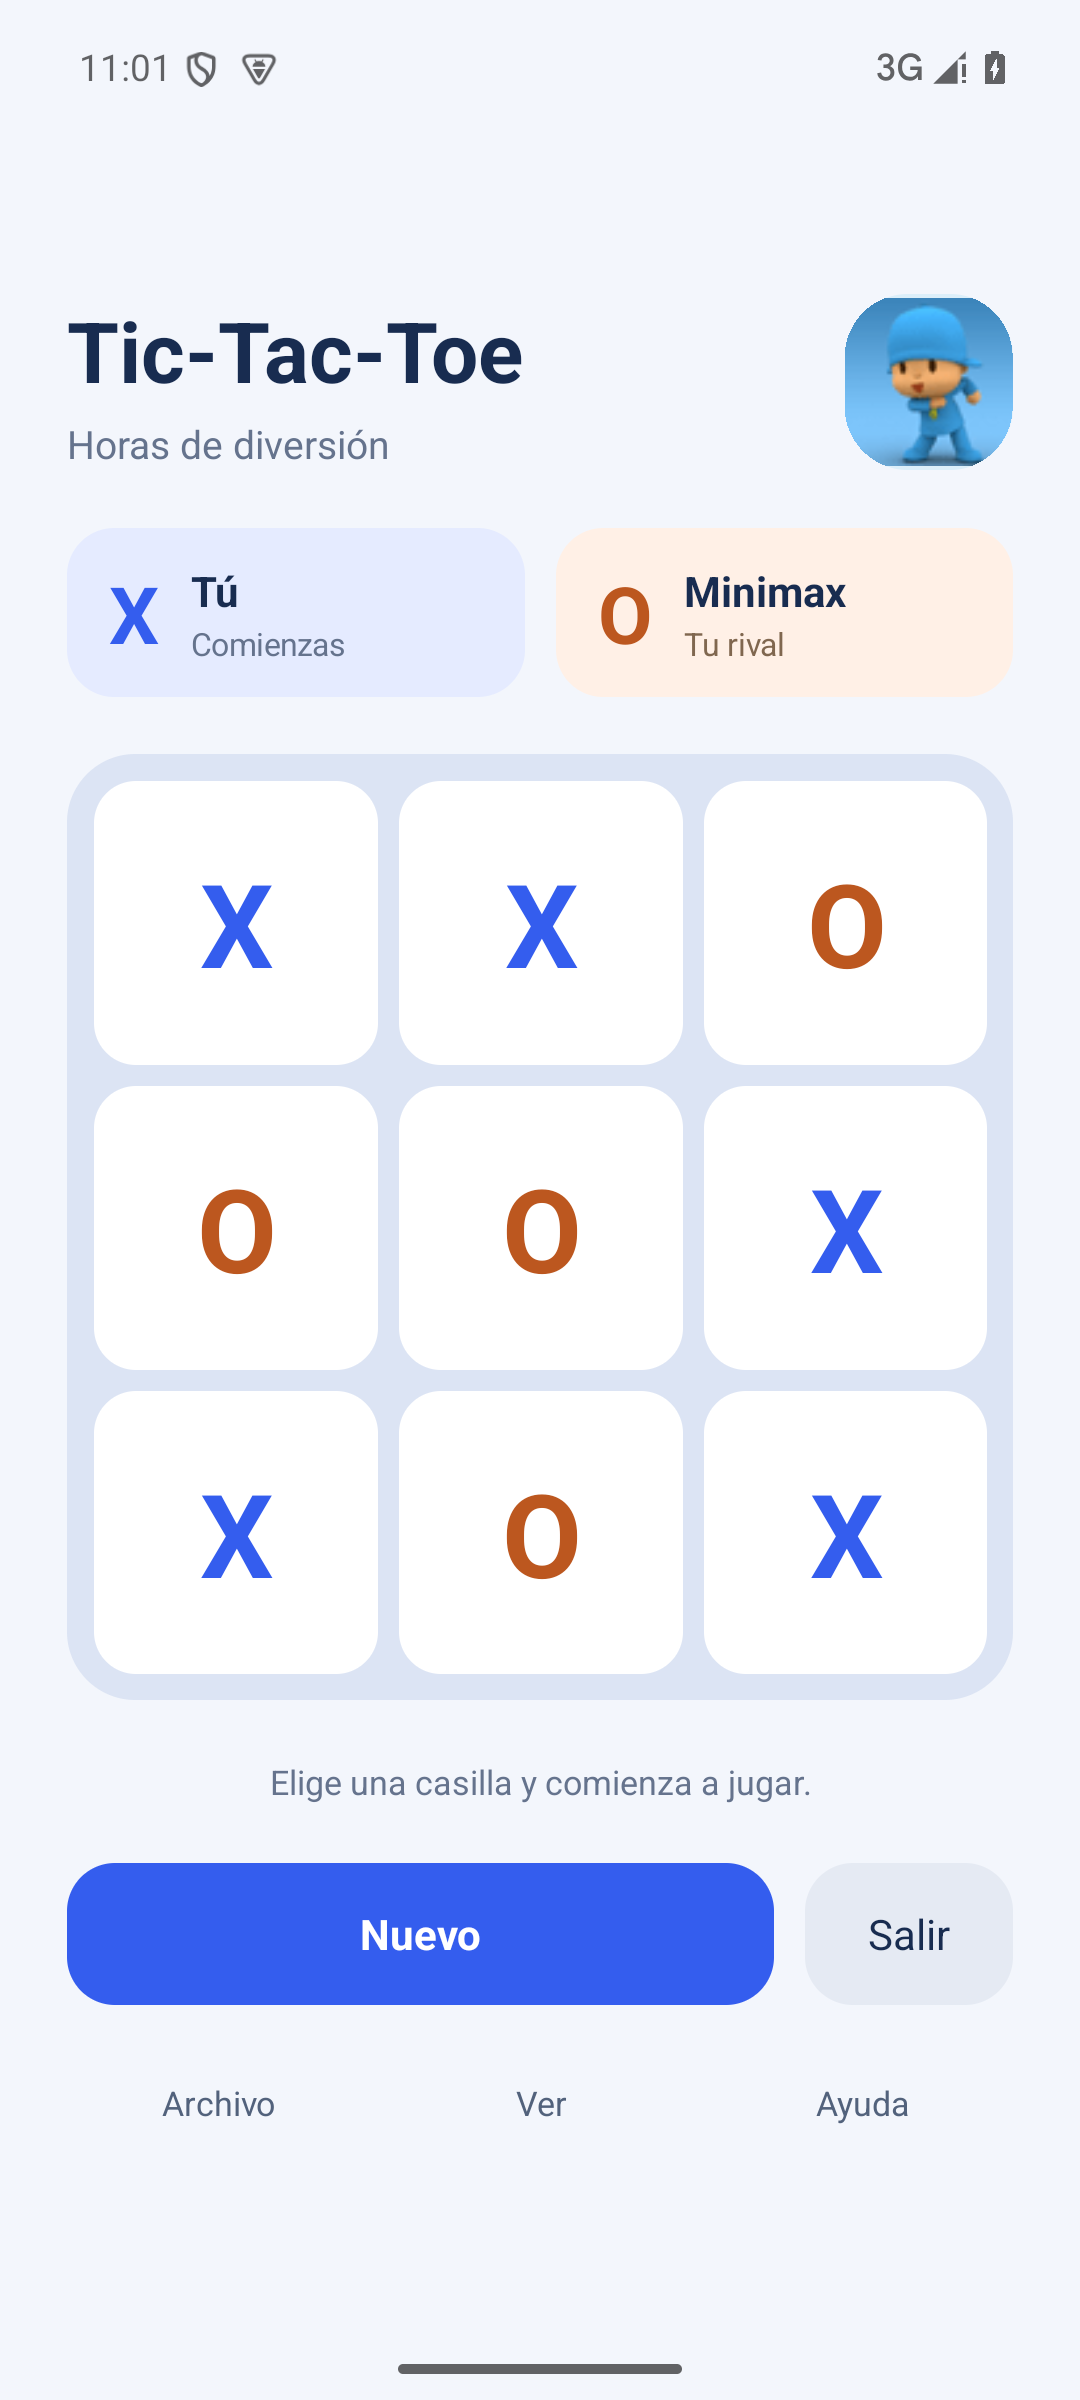
\includegraphics[height=0.65\textheight,keepaspectratio]{capturas_20261104_175826/12_empate_tablero.png}
  \caption{Tablero final de empate entre X y Minimax.}
  \label{fig:minmax-12}
\end{figure}

\begin{figure}[htbp]
  \centering
  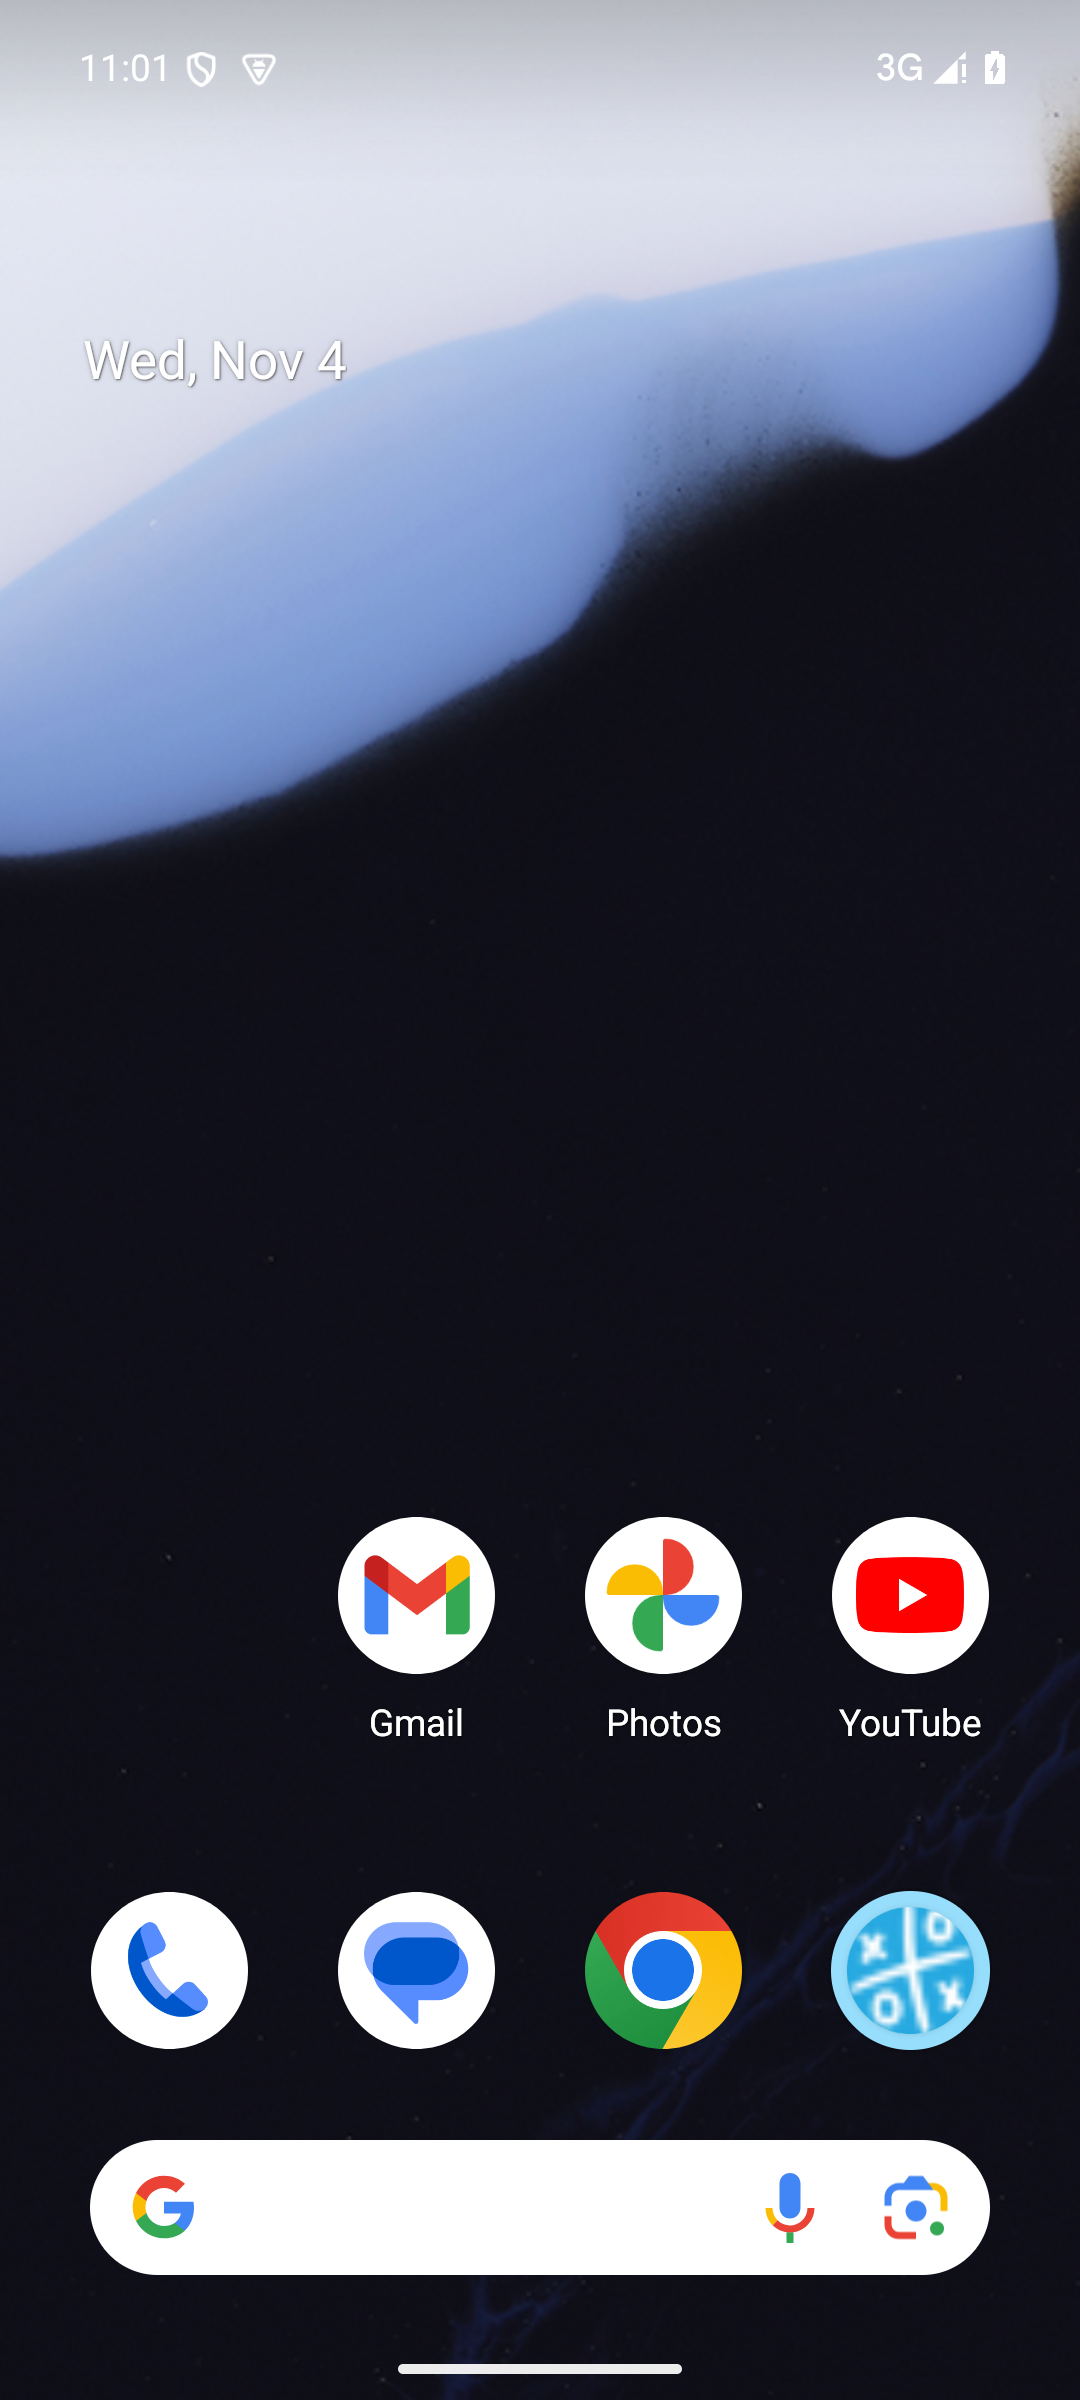
\includegraphics[height=0.65\textheight,keepaspectratio]{capturas_20261104_175826/13_salida.png}
  \caption{Pantalla de inicio Android después de cerrar la aplicación con Salir.}
  \label{fig:minmax-13}
\end{figure}

\begin{figure}[htbp]
  \centering
  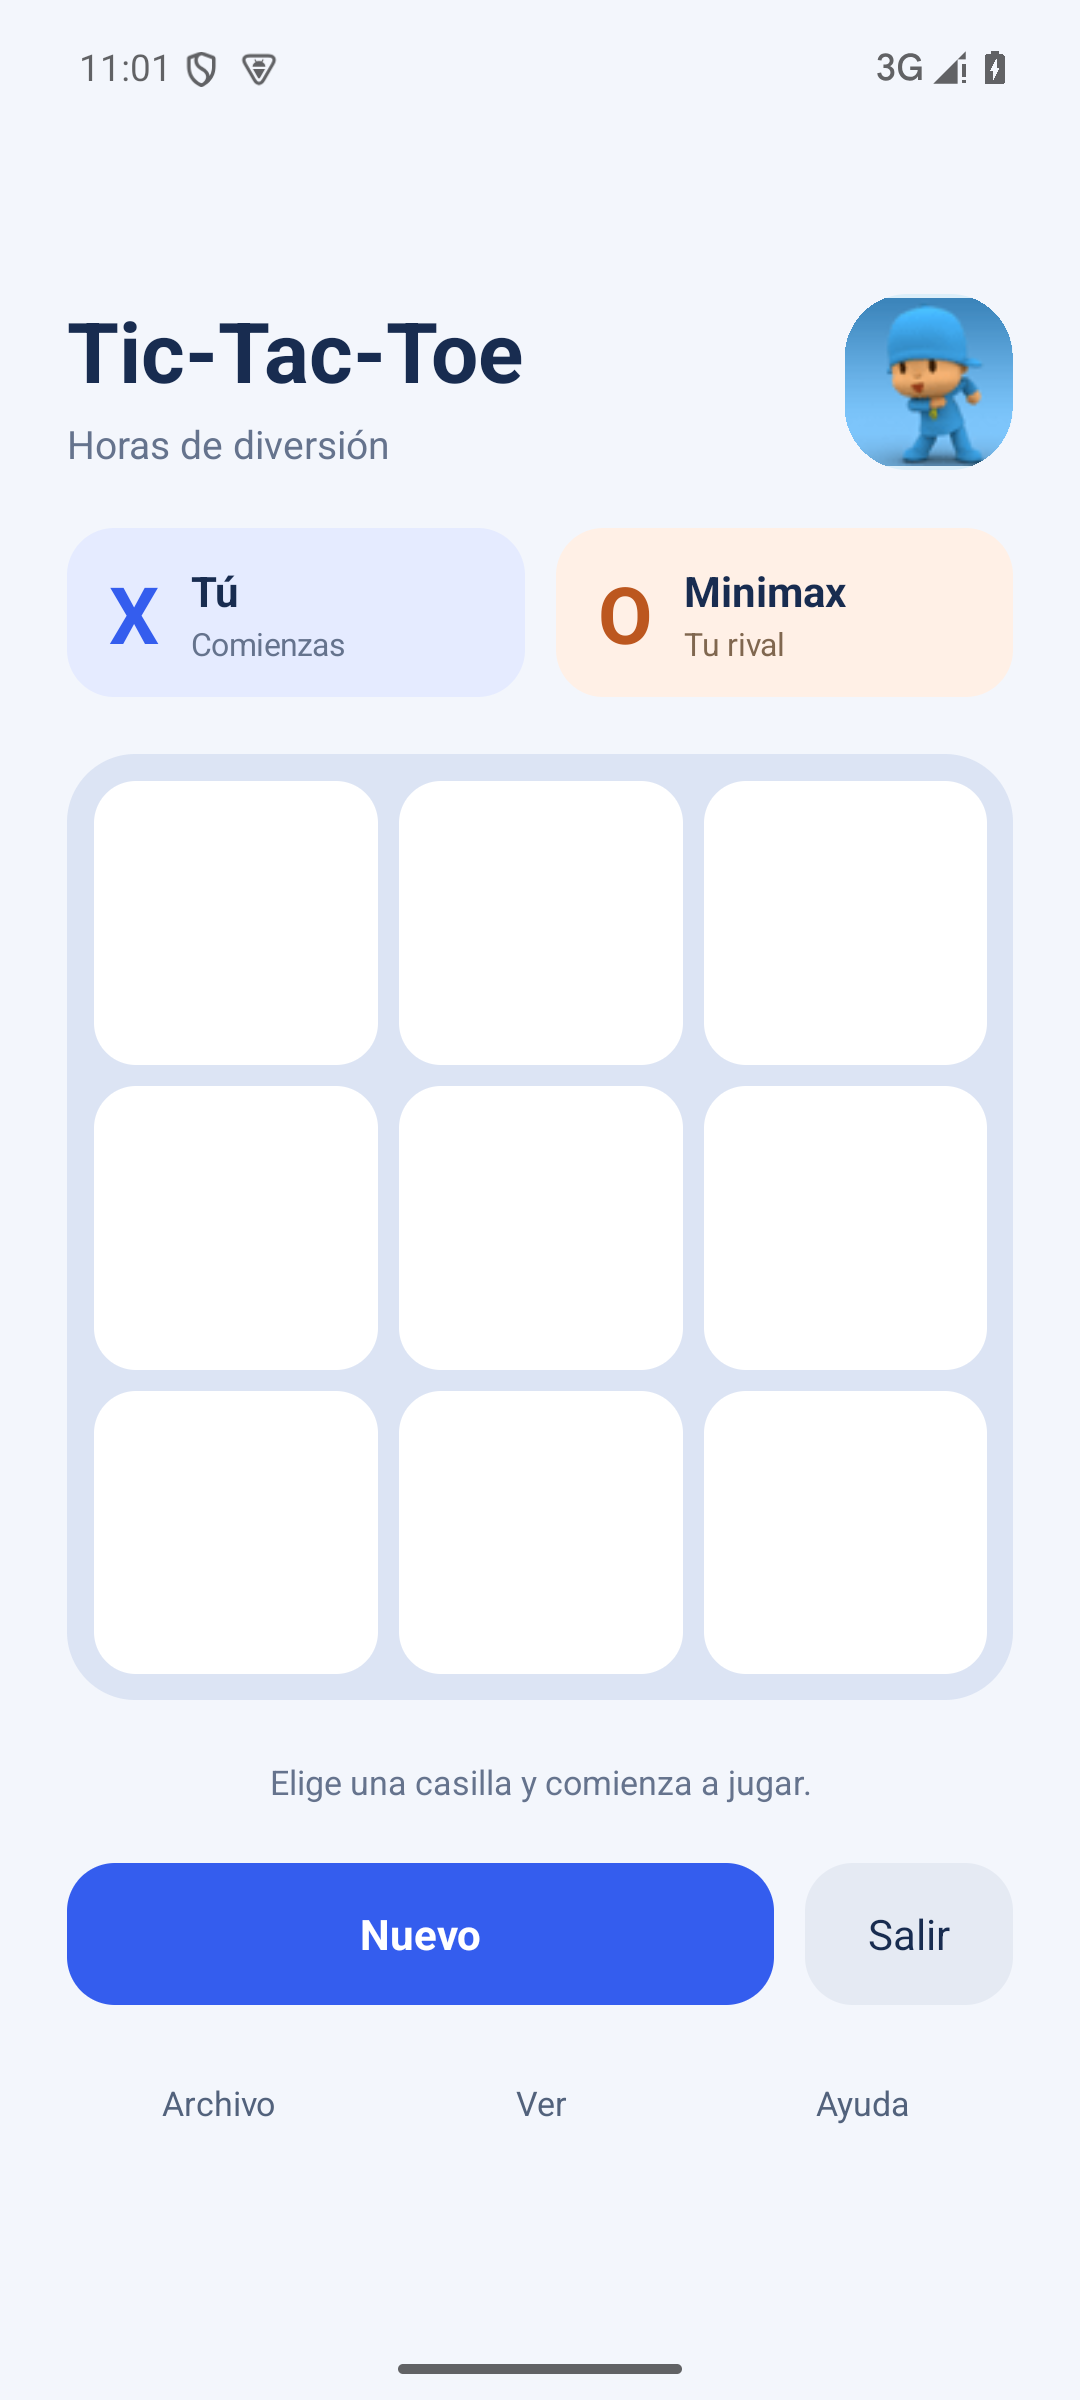
\includegraphics[height=0.65\textheight,keepaspectratio]{capturas_20261104_175826/14_reapertura.png}
  \caption{Aplicación reabierta en el emulador con una partida nueva.}
  \label{fig:minmax-14}
\end{figure}
